\documentclass[11pt]{article}

\usepackage{arxiv}
\usepackage[utf8]{inputenc}
\usepackage[T1]{fontenc}
\usepackage{hyperref}
\usepackage{url}
\usepackage{booktabs}
\usepackage{amsfonts}
\usepackage{amsmath}
\usepackage{amssymb}
\usepackage{nicefrac}
\usepackage{graphicx}
\usepackage{xcolor}
\usepackage{multirow}
\usepackage{subcaption}
\usepackage{enumitem}
\usepackage{float}
\usepackage{needspace}
\usepackage{cleveref}
\usepackage[numbers,sort&compress]{natbib}
\usepackage{tikz}
\usetikzlibrary{positioning,arrows.meta,shapes.geometric,fit,calc,backgrounds}
\usepackage{pgfplots}
\pgfplotsset{compat=1.18}
\usepgfplotslibrary{groupplots}
\usepgfplotslibrary{fillbetween}

\hypersetup{colorlinks=true, linkcolor=blue!50!black, citecolor=blue!50!black, urlcolor=blue!50!black}
\emergencystretch=3em
\hyphenpenalty=1000
\tolerance=2000

% ---- palette (validated: CVD-safe, worst adjacent pair dE 31.9) ----
% blue  = grounded / external / reviewed  (the hero hue)
% orange= internal / ungrounded           (the bounded family)
% red   = second internal series
% violet= distilled student
\definecolor{cGnd}{HTML}{2A78D6}    % grounded / external (blue)
\definecolor{cGndDk}{HTML}{1B5A9E}  % second external series (darker blue, same family)
\definecolor{cUng}{HTML}{EB6834}    % ungrounded / internal (orange)
\definecolor{cUngDk}{HTML}{D1495B}  % second internal series (red)
\definecolor{cStu}{HTML}{4A3AA7}    % distilled student (violet)
\definecolor{cInk}{HTML}{262626}    % primary ink
\definecolor{cMut}{HTML}{6E6E6E}    % secondary ink
\definecolor{cGrid}{HTML}{DDDDDD}   % hairline grid

% ---- shared figure styling: open frame, hairline solid grid, thin marks ----
\pgfplotsset{
  every axis/.append style={
    font=\small,
    axis line style={draw=cMut!70, line width=0.5pt},
    tick style={draw=cMut!70, line width=0.5pt},
    label style={font=\footnotesize, color=cInk},
    tick label style={font=\footnotesize, color=cMut},
    major grid style={solid, cGrid, line width=0.4pt},
    legend style={font=\footnotesize, draw=none, fill=white, fill opacity=0.85, text opacity=1},
  },
  paperbar/.style={% open frame for bar charts: left+bottom spines only
    axis x line*=bottom, axis y line*=left,
  },
  % single clean swatch for bar-chart legends (default ybar legend draws doubled bars)
  swatch/.style={legend image code/.code={%
    \draw[##1] (0cm,-0.09cm) rectangle (0.28cm,0.14cm);}},
  lineswatch/.style={legend image code/.code={%
    \draw[##1] (0cm,0.03cm) -- (0.42cm,0.03cm);}},
}
% direct-label helper for line endpoints
\newcommand{\serieslabel}[3]{\node[font=\scriptsize, anchor=west, text=#1, inner sep=1.5pt] at (axis cs:#2) {#3};}

\title{Grounding the Loop on Both Sides:\texorpdfstring{\\}{ }Interaction as a Third Test-Time Compute Axis,\texorpdfstring{\\}{ }and Why Its Gains Are Invisible\texorpdfstring{\\}{ }Without Grounded Evaluation}

\author{%
  \begin{tabular}{@{}c@{\hspace{4em}}c@{}}
    Bojie Li & Noah Shi \\
    Pine AI & University of Washington
  \end{tabular}%
}
\date{}
\runningtitle{Grounding the Loop on Both Sides}

\begin{document}
\maketitle

\begin{abstract}
Test-time compute is scaled today along two axes---longer \emph{reasoning} and more \emph{sampling}---that share a hidden property: both are \emph{internal}. Every additional token is generated from the same frozen weights and the same prompt, so neither axis can tell the model anything it does not already know. A third axis, \emph{interaction}---propose an artifact, observe it with an external instrument, revise---is not subject to that internal ceiling, because each cycle imports a real observation of the artifact's behavior.

We argue that a single variable, \textbf{grounding}, governs this third axis, and that it must hold on \emph{both} sides of the loop: the feedback that drives revision must come from an instrument that actually observes the defect, and so must the metric that scores the result. We state the argument in one paragraph of information theory (formalized in the appendix) and then test it experimentally. On hard coding tasks at a matched token budget, reasoning-only and best-of-$N$ scaling saturate---the latter even with an \emph{oracle} verifier---while every interaction strategy keeps climbing, the proposer--reviewer harness reaching a strict $100\%$ pass rate with zero seed variance, an effect that replicates across three model families and a held-out suite. On rendered visual artifacts we show that the standard vision--language-model judge is \emph{structurally blind} to the defects the loop fixes---it rates $14$ of $15$ broken single-shot figures ``perfect''---while a deterministic DOM-geometry instrument reveals $40$--$74\%$ defect reductions across four modalities, every one statistically decisive. Swapping only the reviewer's instrument exposes the same asymmetry on the feedback side: a VLM reviewer makes slide layout \emph{worse}, while a geometric reviewer repairs it. Finally, the harness's behavior partially distills into an $8$B student. Interaction scaling is real, distinct from reasoning and sampling, and predictable---but its gains are visible only when both the feedback and the metric are grounded.
\end{abstract}
\begin{center}
\small
Code, task suites, prompts, and deterministic instruments: \url{https://github.com/19PINE-AI/interaction-scaling} \\[2pt]
Website (with an interactive single-shot-vs-reviewed results browser): \url{https://01.me/research/interaction-scaling}
\end{center}
\vspace{-0.6em}

\section{Introduction}
\label{sec:intro}

Scaling test-time compute has become the dominant lever for improving large models on artifact-producing tasks: code, web pages, slides, figures, animations, video edits, research reports. The literature has formalized two axes. \emph{Reasoning scaling} \citep{wei2022chain,yao2023tree,deepseek2025r1,snell2024scaling} spends more tokens thinking before committing to an answer. \emph{Sampling scaling} \citep{wang2023selfconsistency,brown2024large} draws more independent attempts and selects one. The two look different, but they share a property that this paper treats as fundamental: both are \textbf{internal}. Every additional token, whether spent on a longer chain of thought or another sample, is generated from the same frozen weights and the same fixed prompt. More internal compute reorganizes information the system already has; it imports none.

\begin{figure}[t]
\centering
\resizebox{\linewidth}{!}{%
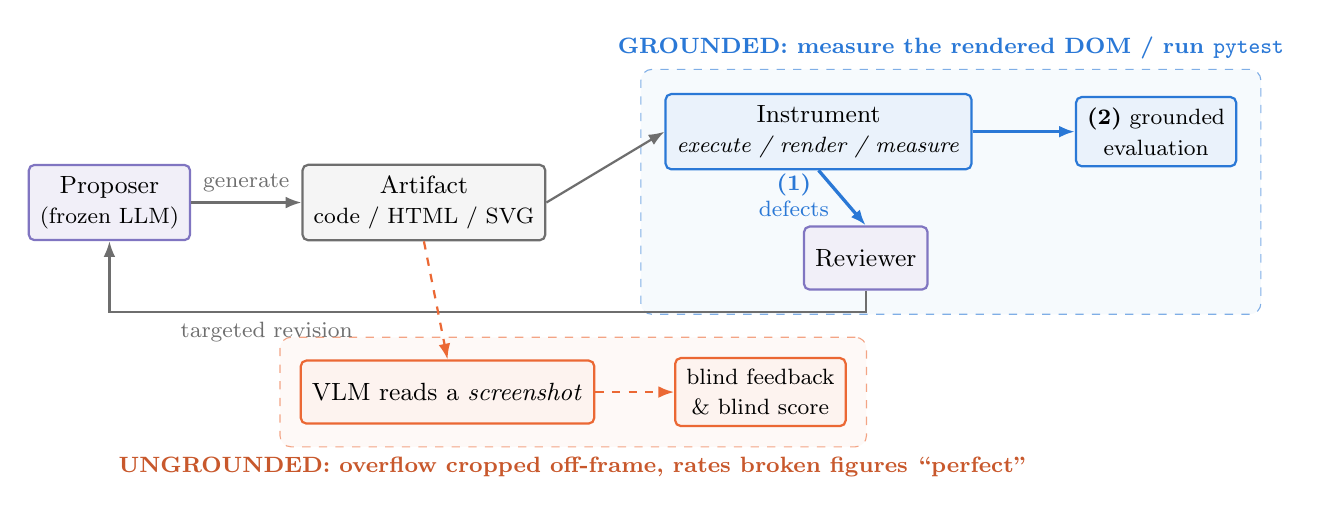
\begin{tikzpicture}[font=\small,
  box/.style={rounded corners=2pt,draw=cMut,thick,minimum height=8mm,align=center,fill=white,inner sep=4pt},
  prop/.style={box,fill=cStu!8,draw=cStu!70},
  env/.style={box,fill=black!4},
  gnd/.style={box,fill=cGnd!10,draw=cGnd},
  ung/.style={box,fill=cUng!8,draw=cUng},
  ar/.style={-{Latex[length=2mm]},thick,cMut},
  gar/.style={-{Latex[length=2mm]},very thick,cGnd},
  uar/.style={-{Latex[length=2mm]},thick,cUng,dashed}]
  \node[prop] (prop) {Proposer\\\footnotesize(frozen LLM)};
  \node[env, right=14mm of prop] (art) {Artifact\\\footnotesize code / HTML / SVG};
  % GROUNDED lane (top)
  \node[gnd, right=15mm of art, yshift=9mm] (inst)
     {Instrument\\\footnotesize\emph{execute / render / measure}};
  \node[gnd, right=13mm of inst] (score) {\footnotesize\textbf{(2)} grounded\\\footnotesize evaluation};
  \node[prop, below=7mm of inst, xshift=6mm] (rev) {Reviewer};
  % UNGROUNDED lane (bottom)
  \node[ung, below=15mm of art, xshift=3mm] (vlm) {VLM reads a \emph{screenshot}};
  \node[ung, right=10mm of vlm] (uscore) {\footnotesize blind feedback\\\footnotesize \& blind score};
  % loop arrows
  \draw[ar] (prop) -- node[above,font=\footnotesize]{generate} (art);
  \draw[ar] (art.east) -- (inst.west);
  \draw[gar] (inst) -- (score);
  \draw[gar] (inst.south) -- node[left,font=\footnotesize,cGnd,align=center,pos=0.45]{\textbf{(1)}\\defects} (rev.north);
  \draw[ar] (rev.south) |- ([yshift=-9mm]art.south) -| node[pos=0.25,below,font=\footnotesize]{targeted revision} (prop);
  % ungrounded branch
  \draw[uar] (art.south) -- (vlm.north);
  \draw[uar] (vlm) -- (uscore);
  \begin{scope}[on background layer]
    \node[draw=cGnd!60,dashed,rounded corners,fill=cGnd!4,fit=(inst)(score)(rev),inner sep=3mm,
      label={[cGnd,font=\footnotesize\bfseries]above:GROUNDED: measure the rendered DOM / run \texttt{pytest}}] {};
    \node[draw=cUng!60,dashed,rounded corners,fill=cUng!4,fit=(vlm)(uscore),inner sep=2.5mm,
      label={[cUng!85!black,font=\footnotesize\bfseries]below:UNGROUNDED: overflow cropped off-frame, rates broken figures ``perfect''}] {};
  \end{scope}
\end{tikzpicture}}
\caption{\textbf{Grounding must hold on both sides of the interaction loop.} A proposer emits an artifact, and a grounded instrument \emph{executes, renders, or measures} it. That single observation does double duty. \textbf{(1)} As grounded \emph{feedback}, it becomes a defect list the reviewer turns into a targeted revision---the channel that lets interaction import information from outside the weights and escape the internal ceiling (\Cref{sec:framework}). \textbf{(2)} As grounded \emph{evaluation}, it is the score that makes the gain measurable. Substituting the default VLM-on-a-screenshot judge (orange lane) breaks \emph{both}: a screenshot drops off-canvas overflow and fine overlap before the model ever sees them, so it neither scores the defect nor---as a reviewer---fixes it.}
\label{fig:concept}
\end{figure}

A third axis breaks this closure: \emph{interaction} with an external instrument that observes the artifact itself---run the tests, render the page and measure the layout, issue the search query. Such an observation is not a function of the weights. It reports how the artifact actually behaves, and it can carry information the model never had. This axis is well established empirically \citep{shinn2023reflexion,yao2023react,gou2024critic,shen2025thinking}, but accounts of \emph{why} and \emph{when} it should beat internal scaling remain informal and, we argue, half-stated. Practitioner reports at industrial scale sharpen the stakes: in a controlled $900$-run deployment study at ByteDance, frontier coding models pass the functional-correctness bar yet miss on delivery quality until a feedback ``harness'' is added---and that report had to invent a multi-axis quality metric before the gap was even visible \citep{hong2026aicoding}. That is a field observation of exactly the two-sided problem we formalize below (detailed in \Cref{sec:related}).

\paragraph{Grounding is the variable, on both sides of the loop.} Our thesis is that one variable governs interaction scaling: \textbf{grounding}---the property that a feedback signal is produced by an instrument observing the artifact's actual form or behavior, rather than by a model rendering an opinion about it. And grounding must hold on \emph{both} sides of the proposer--reviewer loop (\Cref{fig:concept}):
\begin{enumerate}[leftmargin=1.4em,itemsep=1pt,topsep=2pt]
\item \textbf{Grounded feedback} (the signal that drives revision): run the code and read the failing test, render the HTML and measure its bounding boxes, issue the query and read the result. This is the side prior work emphasizes, and a one-paragraph information argument (\Cref{sec:framework}) says it is exactly what lets interaction escape the ceiling that bounds reasoning and sampling.
\item \textbf{Grounded evaluation} (the metric that \emph{measures} the gain): the same observation, used as the score. This side is almost always overlooked, and getting it wrong silently hides the effect.
\end{enumerate}
The second point is not a detail. The default evaluator for visual artifacts is a vision--language model (VLM) reading a screenshot, and a screenshot is an instrument whose channel \emph{drops the defect before the judge ever sees it}: content overflowing the canvas is cropped off-frame, and small overlaps fall below the model's visual acuity. On dense academic figures this judge rates $14$ of $15$ single-shot renders ``perfect'' when a deterministic measurement finds only $3$ actually clean (\Cref{sec:grounded_eval}). Worse, when the same VLM is used as the \emph{reviewer}, its edits make slide layouts worse (\Cref{sec:feedback}). Ungrounded on either side, the third axis either does not fire or cannot be seen.


\Needspace*{6\baselineskip}
\paragraph{Contributions.}
\begin{enumerate}[leftmargin=1.4em,itemsep=1pt,topsep=2pt]
\item \textbf{A grounding framework (\Cref{sec:framework}).} A two-category feedback taxonomy---\emph{ungrounded} model opinion vs.\ \emph{grounded} instrument observation---together with a \emph{coverage} principle: grounded feedback helps exactly as far as the instrument's observational reach. A one-paragraph information argument (formal statement in \Cref{app:ceiling}) explains why internal scaling saturates, and a symmetric observation says an ungrounded \emph{metric} cannot measure the gain. Beyond the documented \emph{biases} of model-as-judge evaluation \citep{zheng2023judging}, we isolate a sharper failure: for artifacts whose quality is a measurable physical property, a screenshot judge is \emph{structurally blind}---not merely noisy---which silently hides a real interaction-scaling effect.
\item \textbf{Interaction keeps scaling where internal compute stops (\Cref{sec:interaction}).} At a matched token budget, reasoning-only and best-of-$N$ saturate---the latter even with an oracle verifier---while every interaction strategy approaches a perfect pass rate, the proposer--reviewer harness doing so at the lowest token cost with zero seed variance.
\item \textbf{The feedback instrument must observe the defect (\Cref{sec:feedback}).} Holding the task suite fixed and swapping only the reviewer's instrument: execution feedback converges far cheaper than critique on behavioral bugs; a linter (grounded, but observing only form) buys nothing on them; and a screenshot-reading VLM reviewer makes slide geometry \emph{worse} while a geometric reviewer repairs it.
\item \textbf{So must the metric (\Cref{sec:grounded_eval}).} The standard VLM judge passes $14$ of $15$ broken figures; a deterministic DOM-geometry instrument instead reveals large, statistically decisive defect reductions under grounded feedback across four visual modalities measured identically---gains the standard metric cannot even see.
\item \textbf{Robustness and internalization (\Cref{sec:robustness,sec:distill}).} The effects replicate across three model families (including the geometry result with Gemini~3.1~Pro as proposer), on a held-out suite, and across a budget-allocation sweep. The harness's behavior also partially distills into an $8$B student at ${\sim}10\times$ lower deployment cost.
\end{enumerate}

\section{The Grounded-Feedback Framework}
\label{sec:framework}

Our contribution is not a new self-correction method but an account of \emph{why} interaction is a separate axis, \emph{when} it helps (a feedback-actionability taxonomy), and a previously-missing requirement: that the \emph{evaluation} be grounded too, without which the effect is unmeasurable.

\subsection{A feedback taxonomy by grounding}
We classify the reviewer's feedback channel by how much external, task-conditional information it injects:
\begin{itemize}[leftmargin=1.4em,itemsep=1pt,topsep=2pt]
\item \textbf{Type 0 -- none.} Single-shot, no feedback.
\item \textbf{Type 1 -- ungrounded critique.} An LLM/VLM critiques the artifact from its weights (``looks wrong''). No execution, no measurement.
\item \textbf{Type 2 -- static analysis.} Linters/type-checkers: signal about the artifact's \emph{form}, not its behavior.
\item \textbf{Type 3 -- grounded.} The artifact is exercised and the result observed: \textbf{3a} execution (run tests, read tracebacks), \textbf{3b} rendered geometry (measure the DOM), \textbf{3c} temporal (sample animation frames), \textbf{3d} factual (search and verify claims).
\end{itemize}

\subsection{Why grounding breaks the ceiling: a DPI bound}
Let $A^\star$ be the (task-determined) correct artifact and $A$ a candidate. The proposer is a channel from its inputs $\Theta$ (weights) and prompt $X$ to $A$. A \emph{reviewer} that only reads $A$ and reasons forms the Markov chain $A^\star \to (\Theta,X) \to A \to R$, where $R$ is its critique. By the data-processing inequality,
\[
I(A^\star; R)\ \le\ I(A^\star; (\Theta,X)),
\]
so \emph{no} amount of reasoning or ungrounded review (Type 0--2) can recover more information about $A^\star$ than is already in $(\Theta,X)$. This bounds reasoning-only scaling. Sampling is bounded differently but no less tightly: for any finite $N$, best-of-$N$ can only \emph{select} among the $N$ candidates the proposer actually draws, so even an oracle (grounded) verifier cannot return a correct artifact the proposer is too unlikely to sample within the budget. Its practical ceiling is the high-probability support of the proposer's own output distribution, not a new information channel. Both ceilings appear empirically once we measure them (\Cref{fig:dpi} in \Cref{sec:interaction}): on hard code, both reasoning-only and oracle best-of-$N$ saturate well short of completion. The inequality bounds the \emph{information channel}, not achievable quality directly; we use it to \emph{motivate} the saturation we then measure and treat as the evidence.

Grounded feedback (Type 3) escapes both ceilings by feeding an environment observation $E=g(A,\,\mathrm{world})$ (a test outcome, a measured bounding box, a search verdict) back into \emph{generation}. Conditioning the next proposal on $E$ lets the proposer synthesize a candidate it would not otherwise have sampled: formally $I(A^\star;(R,E))$ can exceed $I(A^\star;(\Theta,X))$ because $E$ carries information obtained by \emph{running} the artifact against reality. This is the crucial difference from selection (best-of-$N$ cannot create a missing candidate) and from reasoning (which adds no information), and it is why interaction is a distinct axis rather than a constant-factor speedup.

\paragraph{The symmetric claim: ungrounded evaluation cannot measure the gain.} The same inequality applies to the \emph{scorer}. A metric $M$ that is itself a function of $(\Theta,X)$ (e.g.\ a VLM judging a screenshot, whose view of $A$ is a lossy, cropped image) satisfies $I(A^\star; M)\le I(A^\star;(\Theta,X))$ and cannot certify an improvement that lives in the part of $A$ it cannot observe. Grounding the evaluation (measure the artifact directly) is therefore not optional polish: it is a precondition for \emph{detecting} interaction scaling on any modality whose quality is not fully visible to the default judge. \Cref{sec:grounded_eval} shows this is exactly the situation for rendered visual artifacts.

\subsection{Predictions}
The framework makes three testable predictions, each tested below. \textbf{(P1)} Reasoning- and sampling-only scaling saturate strictly below the interaction ceiling (\Cref{sec:interaction}). \textbf{(P2)} Within interaction, more actionable grounded channels lift more, and the \emph{execution} of the artifact, not the extra review pass, is the active ingredient (\Cref{sec:interaction}). \textbf{(P3)} On modalities whose quality is invisible to the default judge, the gain is only detectable with a grounded metric, and an ungrounded reviewer can even regress quality (\Cref{sec:grounded_eval}).

\section{Setup: A Budget-Aware Proposer--Reviewer Harness}
\label{sec:method}

\paragraph{Architecture.} The harness is pure scaffolding around a \emph{frozen} frontier model (Claude Sonnet~4, \texttt{claude-sonnet-4-20250514}, temperature~$0$ unless noted): no fine-tuning, no retrieval, no learned controller. A \textbf{proposer} produces an artifact. An \textbf{instrument} executes, renders, or measures it to produce a grounded signal. A \textbf{reviewer} (the same model in a diagnostic role) turns that signal into a structured list of defects, and the proposer revises. The loop repeats up to an iteration cap and \emph{keeps the best-scoring iteration}, so the reviewed result can never score below single-shot under the same metric. Single-shot is just one proposer call.

\paragraph{The three grounded instruments.} Every modality is paired with a deterministic or near-deterministic instrument that both \emph{feeds back} and \emph{scores}:
\begin{itemize}[leftmargin=1.4em,itemsep=1pt,topsep=2pt]
\item \textbf{Execution} (\texttt{pytest}): exact pass/fail plus the failing assertion and traceback. Each task ships a multi-assertion suite targeting the edge cases that separate correct from plausible-but-wrong (e.g.\ the semantic-version comparator is checked on pre-release precedence), and the deep-spec suite is additionally validated against a reference implementation. A ``pass'' therefore certifies the specified behavior, and the oracle best-of-$N$ baseline of \Cref{sec:interaction} selects against these \emph{same} tests, so its ceiling is measured by the identical criterion.
\item \textbf{Rendered geometry}: the artifact is rendered headless and every element's true bounding box is read from the layout engine. We compute, exactly: text-on-text overlap ($\ge 6$\,px), out-of-bounds/clipping, container overflow, document overflow ($>16$\,px), and \emph{box-group misalignment} (rows or columns of card-like boxes flagged for unequal size, misaligned far edges, or uneven gutters). Web pages are scored at desktop and mobile widths; animations are probed at each sampled frame.
\item \textbf{Native video} (Gemini~3.1~Pro): the rendered clip is judged whole against per-requirement binary checks, a near-grounded substitute where pixels, not a still, are observed.
\end{itemize}
Where no deterministic instrument exists (flowing web content, factual research), we fall back to a binary per-requirement rubric, flagged as such.

\begin{table}[t]
\centering
\small
\caption{Modality instantiations. Each modality pairs a grounded feedback channel (named per the taxonomy of \Cref{fig:taxonomy}) with the instrument that both drives revision and scores the result. ``$\dagger$'' marks the four modalities scored by the deterministic DOM-geometry instrument and analyzed jointly in \Cref{sec:grounded_eval}.}
\label{tab:setup}
\begin{tabular}{llll}
\toprule
Modality & Feedback channel & Grounded instrument & Hard suite ($N$) \\
\midrule
Code             & execution     & \texttt{pytest} pass/fail + traceback   & $15$ (+$11$ deep-spec) \\
Academic figures$^\dagger$ & geometry & DOM geometry + alignment           & $20$ \\
Slides$^\dagger$           & geometry & DOM geometry + alignment           & $12$ real-paper \\
Web pages$^\dagger$        & geometry & DOM geometry, multi-width          & $20$ \\
Animations$^\dagger$       & temporal & DOM geometry, per-frame            & $20$ SVG/CSS \\
Video editing    & exec.\ + temporal & script exec + Gemini-native rubric & $15$ \\
Deep research    & external facts & search-grounded factual rubric         & $15$ \\
\bottomrule
\end{tabular}
\end{table}

All artifacts are produced under a common \emph{design-principle} generation prompt (proximity, alignment, repetition, contrast, deliberate color) so that single-shot quality is already strong: the headroom we measure reflects genuine task difficulty, not a weak prompt.

\paragraph{Budget and protocol.} A run has a token budget $B$ split across proposer and reviewer calls; \Cref{sec:robustness} sweeps the split, and \Cref{tab:setup} lists the per-modality instruments. Unless noted, the proposer runs at temperature $0$, and each modality is evaluated over three independent seeds, keeping the best-scoring iteration (cap $\le 3$ for geometry, $\le 5$ for code); we compare single-shot against reviewed on each (task, seed) pair. For each result we report a two-sided paired sign test over the decisive pairs and, for the geometry and code effects, a paired-bootstrap $95\%$ confidence interval on the effect size; exact values accompany each figure.

\section{Interaction Scaling at a Matched Token Budget}
\label{sec:interaction}

\paragraph{The saturation experiment (P1).} On the hard code suite, at a fixed per-task token budget, we compare four strategies: reasoning-only (extended thinking), best-of-$N$ sampling with an \emph{oracle} verifier, a single-agent loop, and the proposer--reviewer harness. The result is \Cref{fig:scaling}, previewed in \Cref{sec:ceiling}: both internal strategies flatten as the budget grows, while \emph{every} strategy that iterates on feedback climbs past them toward a perfect pass rate. The best-of-$N$ comparison is the sharpest, because its verifier is the ground-truth test suite itself, so its ceiling is effectively pass@$N$: the tasks it never solves are those where none of its samples passes, and a perfect selector cannot return a candidate the proposer never writes. The harness solves those same tasks by conditioning the next draw on execution feedback. The gap is information-theoretic, not a tuning artifact.

\paragraph{Code as the clean case study.} Code is the cleanest demonstration, because the instrument is exact and the score is objective. The harness recovers every first-shot failure with no regressions, on both the development suite and a harder deep-spec suite of from-scratch implementations (a JSON parser, a spreadsheet-reference resolver, a minimal edit-script diff, an expression evaluator), lifting both to a perfect $100\%$ pass rate (\Cref{fig:code}). The mechanism is the same across recovered traces: turn~1 produces code that compiles but mishandles an edge case (an off-by-one boundary, semantic-version comparison, CIDR arithmetic); turn~2 receives the failing assertion, the offending input, and the expected-vs-actual values, and rewrites just that block; turn~3 confirms the fix. Reasoning alone cannot supply this: the model cannot know its boundary condition is wrong until a concrete test exercises it.

\begin{figure}[t]
\centering
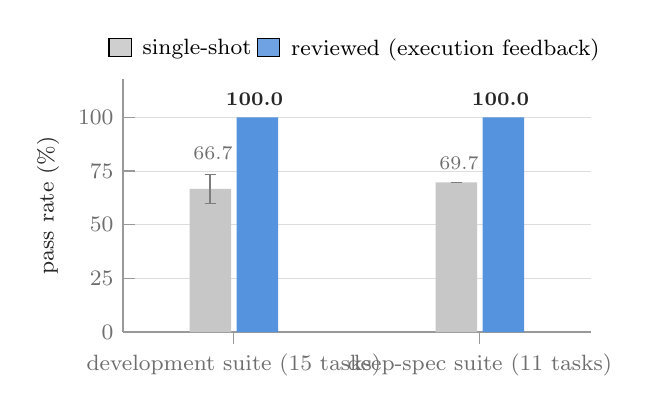
\begin{tikzpicture}
\begin{axis}[paperbar,width=0.62\linewidth,height=4.8cm,
  ybar,bar width=15pt,ymin=0,ymax=118,
  ylabel={pass rate (\%)},
  symbolic x coords={dev,deepspec},xtick=data,
  xticklabels={development suite (15 tasks),deep-spec suite (11 tasks)},
  x tick label style={font=\footnotesize,color=cMut},
  enlarge x limits=0.45,ytick={0,25,50,75,100},ymajorgrids,
  legend style={at={(0.5,1.03)},anchor=south,legend columns=2,
    /tikz/every odd column/.append style={column sep=2pt}}]
  \addplot[swatch,draw=none,fill=black!22,
    error bars/.cd,y dir=both,y explicit,error bar style={cInk!60,line width=0.6pt}]
    coordinates {(dev,66.7) +- (0,6.7) (deepspec,69.7) +- (0,0)};
    \addlegendentry{single-shot}
  \addplot[swatch,draw=none,fill=cGnd!80]
    coordinates {(dev,100) (deepspec,100)};
    \addlegendentry{reviewed (execution feedback)}
  % selective labels: the reviewed endpoints and the lifts
  \node[font=\scriptsize\bfseries,cInk,anchor=south] at (axis cs:dev,101) {\hspace{15pt}100.0};
  \node[font=\scriptsize\bfseries,cInk,anchor=south] at (axis cs:deepspec,101) {\hspace{15pt}100.0};
  \node[font=\scriptsize,cMut,anchor=south] at (axis cs:dev,76) {\hspace{-15pt}66.7};
  \node[font=\scriptsize,cMut,anchor=south] at (axis cs:deepspec,71) {\hspace{-15pt}69.7};
\end{axis}
\end{tikzpicture}
\caption{\textbf{Execution feedback recovers every first-shot failure on both code suites.} Single-shot vs.\ harness-reviewed pass rate (development suite: $3$-seed mean, whisker $\pm1$\,SD; deep-spec: sign test $p=0.002$). Every failing run is recovered and no passing run regresses; the reviewed bars carry zero seed variance.}
\label{fig:code}
\end{figure}

\paragraph{Architecture buys efficiency and reliability, not ceiling.} Among interaction strategies, the ceiling pass rate ties within seed noise; what separates them is cost and variance (\Cref{fig:efficiency}). The proposer--reviewer harness is the most token-efficient, and the only variant that reaches $100\%$ in \emph{every} seed. Three things explain the efficiency: the reviewer sees only what it needs to locate defects, it returns a structured list rather than raw \texttt{stderr}, and the two roles are specialized.

\begin{figure}[t]
\centering
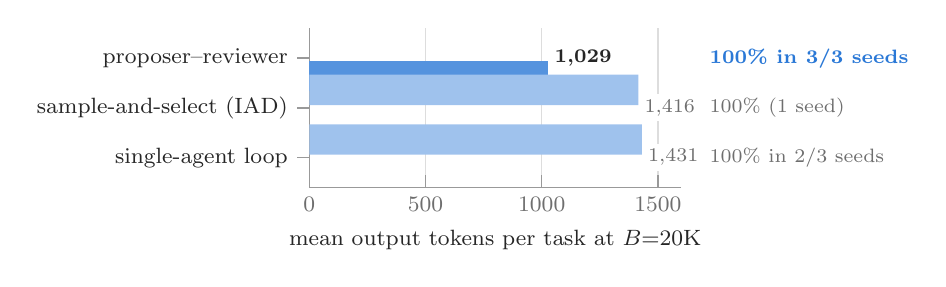
\begin{tikzpicture}
\begin{axis}[paperbar,width=0.52\linewidth,height=3.6cm,
  xbar,xmin=0,xmax=1600,bar width=11pt,enlarge y limits=0.3,
  xlabel={mean output tokens per task at $B{=}20$K},
  symbolic y coords={loop,iad,harness},ytick={loop,iad,harness},
  yticklabels={single-agent loop,sample-and-select (IAD),proposer--reviewer},
  y tick label style={font=\footnotesize,color=cInk},
  xtick={0,500,1000,1500},xticklabels={0,500,1000,1500},xmajorgrids,clip=false]
  \addplot[draw=none,fill=cGnd!80] coordinates {(1029,harness)};
  \addplot[draw=none,fill=cGnd!45] coordinates {(1416,iad) (1431,loop)};
  % token value at each bar tip; reliability as a right-hand column
  \node[font=\scriptsize\bfseries,cInk,anchor=west,inner sep=2pt] at (axis cs:1029,harness) {1{,}029};
  \node[font=\scriptsize,cMut,anchor=west,inner sep=2pt,fill=white] at (axis cs:1416,iad) {1{,}416};
  \node[font=\scriptsize,cMut,anchor=west,inner sep=2pt,fill=white] at (axis cs:1431,loop) {1{,}431};
  \node[font=\scriptsize\bfseries,cGnd,anchor=west] at (axis cs:1680,harness) {100\% in 3/3 seeds};
  \node[font=\scriptsize,cMut,anchor=west] at (axis cs:1680,iad) {100\% (1 seed)};
  \node[font=\scriptsize,cMut,anchor=west] at (axis cs:1680,loop) {100\% in 2/3 seeds};
\end{axis}
\end{tikzpicture}
\caption{\textbf{Same ceiling, different cost and reliability.} All three interaction strategies use execution feedback and tie on pass rate within seed noise (sign test $p>0.6$); the proposer--reviewer harness converges with ${\sim}28\%$ fewer tokens and is the only variant at $100\%$ across all seeds (\Cref{tab:LvsH}).}
\label{fig:efficiency}
\end{figure}

\paragraph{Built-in early stopping.} The loop does not over-revise: on code, \emph{every} already-passing single-shot task is submitted at iteration~1 with no revision and no wasted tokens. The grounded signal (a failing test) is the trigger; without it the loop is silent. This is why the harness's token overhead over single-shot stays modest despite a generous iteration cap.

\section{The Feedback Side: The Instrument Must Observe the Defect}
\label{sec:feedback}

The saturation experiment compared strategies. This section holds everything else fixed---task suite, proposer model, number of reviewing passes---and swaps \emph{only the reviewer's feedback channel}, testing the coverage principle (P2) directly on both a textual and a visual modality.

\paragraph{On code: execution feedback wins where its coverage lies.} We run three arms on the fixed code suite, each with \emph{exactly one} reviewing pass: an ungrounded critique reviewer (the LLM re-reads the code), a static-form reviewer (the same critique plus \texttt{ruff} linter output), and an execution reviewer (the same critique plus the failing test's traceback). Any separation therefore isolates the \emph{signal}, not the act of reviewing. \Cref{fig:typecontrol} shows both outcomes. The pass-rate separation is modest and we read it cautiously, since it rests on a single leaner-budget seed. The unambiguous separation is \emph{cost}: the execution arm converges roughly $2.5\times$ cheaper and in fewer iterations, because a concrete failing assertion localizes the fix where an ungrounded critique gropes. The static-form arm is the coverage principle's cleanest prediction: the linter is a genuinely grounded instrument, but the seeded bugs are runtime-logic errors that leave no trace in form, so it buys nothing over bare critique---grounding helps only as far as the instrument can see.\footnote{Symmetrically, the principle predicts a static-form lift on a bug set that \emph{is} visible in form (type confusions catchable by \texttt{mypy}, taint patterns catchable by \texttt{semgrep}). Constructing that suite is future work; on our behavioral bug set the null result is the prediction.}

\begin{figure}[t]
\centering
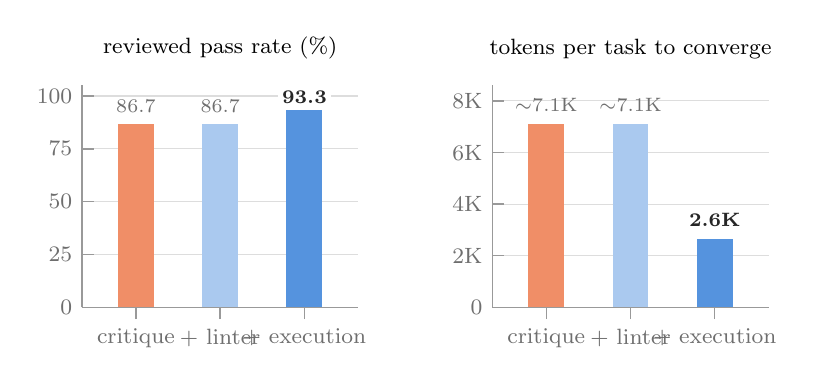
\begin{tikzpicture}
\begin{axis}[paperbar,name=axpass,width=0.42\linewidth,height=4.4cm,
  ybar,bar width=13pt,ymin=0,ymax=105,
  title={\footnotesize reviewed pass rate (\%)},
  symbolic x coords={critique,linter,execution},xtick={critique,linter,execution},
  xticklabels={critique,{+ linter},{+ execution}},
  x tick label style={font=\footnotesize,color=cMut},
  enlarge x limits=0.32,ytick={0,25,50,75,100},ymajorgrids]
  \addplot[draw=none,fill=cUng!75,bar shift=0pt] coordinates {(critique,86.7)};
  \addplot[draw=none,fill=cGnd!40,bar shift=0pt] coordinates {(linter,86.7)};
  \addplot[draw=none,fill=cGnd!80,bar shift=0pt] coordinates {(execution,93.3)};
  \node[font=\scriptsize,cMut,anchor=south] at (axis cs:critique,87.5) {86.7};
  \node[font=\scriptsize,cMut,anchor=south] at (axis cs:linter,87.5) {86.7};
  \node[font=\scriptsize\bfseries,cInk,anchor=south,fill=white,inner sep=1.5pt] at (axis cs:execution,94) {93.3};
\end{axis}
\begin{axis}[paperbar,at={($(axpass.east)+(1.7cm,0)$)},anchor=west,
  width=0.42\linewidth,height=4.4cm,
  ybar,bar width=13pt,ymin=0,ymax=8600,
  title={\footnotesize tokens per task to converge},
  symbolic x coords={critique,linter,execution},xtick={critique,linter,execution},
  xticklabels={critique,{+ linter},{+ execution}},
  x tick label style={font=\footnotesize,color=cMut},
  enlarge x limits=0.32,ytick={0,2000,4000,6000,8000},
  yticklabels={0,2K,4K,6K,8K},ymajorgrids]
  \addplot[draw=none,fill=cUng!75,bar shift=0pt] coordinates {(critique,7100)};
  \addplot[draw=none,fill=cGnd!40,bar shift=0pt] coordinates {(linter,7100)};
  \addplot[draw=none,fill=cGnd!80,bar shift=0pt] coordinates {(execution,2643)};
  \node[font=\scriptsize,cMut,anchor=south] at (axis cs:critique,7200) {$\sim$7.1K};
  \node[font=\scriptsize,cMut,anchor=south] at (axis cs:linter,7200) {$\sim$7.1K};
  \node[font=\scriptsize\bfseries,cInk,anchor=south] at (axis cs:execution,2750) {2.6K};
\end{axis}
\end{tikzpicture}
\caption{\textbf{Swapping only the feedback signal on a fixed code suite: improvement tracks coverage, and cost tracks it decisively.} One reviewing pass per arm. Ungrounded critique (orange), critique + linter (light blue: grounded, but observing only \emph{form}), and critique + test execution (blue: grounded, observing \emph{behavior}). The linter arm matches bare critique on these runtime-logic bugs---exactly what the coverage principle predicts---while the execution arm reaches a higher ceiling at ${\sim}2.5\times$ lower cost and fewer iterations ($1.53$ vs.\ $2.07$; per-seed detail in \Cref{tab:type-controls}).}
\label{fig:typecontrol}
\end{figure}

\paragraph{On slides and figures: an uncovered instrument makes things worse.} The decisive form of the control is visual. We fix the task suite and the proposer, and give the reviewer either (i) the deterministic geometry report---measured boxes, exact overlaps---or (ii) a VLM's reading of a screenshot, an instrument whose channel crops the very defects at issue. Because the two arms are separate runs, each is compared against its \emph{own} single-shot baseline, and the load-bearing contrast is the \emph{direction} each reviewer moves that baseline (\Cref{fig:ablation}). The geometric reviewer sharply reduces real layout defects on both modalities. The VLM reviewer does not: it \emph{increases} defects on slides and is directionally worse on figures. Blind to the true geometry, its edits break alignment about as often as they fix it---one reviewing pass, opposite sign, set entirely by whether the signal's coverage includes the defect. (On the same slides the binary VLM \emph{rubric} simultaneously saturates, which is the evaluation-side half of the story; \Cref{sec:grounded_eval} takes it up.)

\begin{figure}[t]
\centering
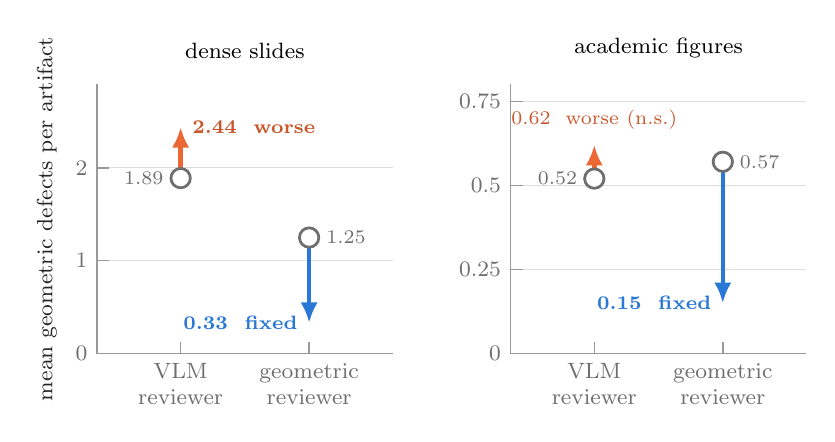
\begin{tikzpicture}[
  dumb/.style={line width=1.6pt,-{Latex[length=2.6mm,width=2.2mm]}},
  ssdot/.style={circle,draw=cMut,fill=white,line width=1pt,inner sep=0pt,minimum size=7pt}]
\begin{axis}[name=axslide,width=0.44\linewidth,height=5.0cm,
  title={\footnotesize dense slides},
  ylabel={mean geometric defects per artifact},
  xmin=0.35,xmax=2.65,ymin=0,ymax=2.9,ytick={0,1,2},
  xtick={1,2},xticklabels={VLM\\reviewer,geometric\\reviewer},
  x tick label style={font=\footnotesize,color=cMut,align=center},
  ymajorgrids,axis x line*=bottom,axis y line*=left]
  % VLM arm: 1.89 -> 2.44 (worse, orange, up)
  \draw[dumb,cUng] (axis cs:1,1.89) -- (axis cs:1,2.44);
  \node[ssdot] at (axis cs:1,1.89) {};
  \node[font=\scriptsize,cMut,anchor=east,inner sep=6pt] at (axis cs:1,1.89) {1.89};
  \node[font=\scriptsize\bfseries,cUng!85!black,anchor=west,inner sep=4pt] at (axis cs:1,2.44) {2.44 \ worse};
  % geom arm: 1.25 -> 0.33 (better, blue, down)
  \draw[dumb,cGnd] (axis cs:2,1.25) -- (axis cs:2,0.33);
  \node[ssdot] at (axis cs:2,1.25) {};
  \node[font=\scriptsize,cMut,anchor=west,inner sep=6pt] at (axis cs:2,1.25) {1.25};
  \node[font=\scriptsize\bfseries,cGnd,anchor=east,inner sep=4pt] at (axis cs:2,0.33) {0.33 \ fixed};
\end{axis}
\begin{axis}[at={($(axslide.east)+(1.5cm,0)$)},anchor=west,
  width=0.44\linewidth,height=5.0cm,
  title={\footnotesize academic figures},
  xmin=0.35,xmax=2.65,ymin=0,ymax=0.8,ytick={0,0.25,0.5,0.75},
  xtick={1,2},xticklabels={VLM\\reviewer,geometric\\reviewer},
  x tick label style={font=\footnotesize,color=cMut,align=center},
  ymajorgrids,axis x line*=bottom,axis y line*=left]
  \draw[dumb,cUng] (axis cs:1,0.52) -- (axis cs:1,0.62);
  \node[ssdot] at (axis cs:1,0.52) {};
  \node[font=\scriptsize,cMut,anchor=east,inner sep=6pt] at (axis cs:1,0.52) {0.52};
  \node[font=\scriptsize,cUng!85!black,anchor=south,inner sep=3pt] at (axis cs:1,0.64) {0.62 \ worse (n.s.)};
  \draw[dumb,cGnd] (axis cs:2,0.57) -- (axis cs:2,0.15);
  \node[ssdot] at (axis cs:2,0.57) {};
  \node[font=\scriptsize,cMut,anchor=west,inner sep=6pt] at (axis cs:2,0.57) {0.57};
  \node[font=\scriptsize\bfseries,cGnd,anchor=east,inner sep=4pt] at (axis cs:2,0.15) {0.15 \ fixed};
\end{axis}
\end{tikzpicture}
\caption{\textbf{Same tasks, same proposer, one reviewing pass---the arrow's direction is set by the reviewer's instrument.} Each arrow runs from that arm's own single-shot baseline (open circle; the arms are separate runs, hence differing baselines) to its reviewed result, in mean geometric defects per artifact (lower is better; note the differing $y$ scales). The screenshot-fed VLM reviewer moves \emph{up} on slides and directionally up on figures; the deterministic geometric reviewer moves sharply \emph{down} on both (slides $-73\%$, $p=0.0018$; figures $-74\%$, $p=7{\times}10^{-4}$).}
\label{fig:ablation}
\end{figure}

\paragraph{What this establishes.} On the feedback side, grounding is necessary but the operative quantity is \emph{coverage}: a grounded instrument that cannot observe the defect class (the linter, on runtime bugs) matches ungrounded critique, and an instrument whose channel actively drops the defect (the screenshot) is worse than no reviewer at all. The remaining question is symmetric: what happens when the \emph{metric} is such an instrument.

\section{Grounding the Evaluation: The Gain Is Invisible to a VLM}
\label{sec:grounded_eval}

The visual modalities expose the symmetric half of the framework (P3): even when grounded feedback \emph{does} fix the artifact, an ungrounded metric cannot see it.

\paragraph{The default VLM judge is structurally blind.} Our starting evaluator is a binary per-requirement rubric scored by a VLM over a screenshot. On $15$ dense academic-paper architecture figures, even with native-resolution quadrant tiling, this judge rates \textbf{$14$ of $15$} single-shot renders ``perfect'', i.e.\ satisfying every \emph{content} requirement it is asked to check (the right components present, labels correct). Layout geometry is simply not a question the screenshot lets it answer. By direct inspection the renders are broken (superimposed section titles, labels spilling out of boxes), so the failure is mechanical, not fixable by prompting the judge better. Screenshots are captured at $1080$\,px, so any content overflowing the canvas is cropped \emph{off-frame before the image reaches the judge} (the defect is literally absent from the pixels the model sees), and small in-frame overlaps fall below its acuity. A deterministic DOM-geometry check finds only \textbf{$3$ of $15$} are actually clean. The $14$-vs-$3$ gap is therefore not a \emph{wrong} answer to the same question but the judge being \emph{structurally unable to observe} the property that matters (\Cref{fig:blind}). (This initial probe is a deliberately hard, unconstrained set. The suite scored in \Cref{tab:geometric} is generated under the design-principle prompt of \Cref{sec:method} and is correspondingly cleaner single-shot, with headroom that is genuine task difficulty surviving a strong prompt, not a weak one.)

\begin{figure}[t]
\centering
\begin{subfigure}[b]{0.35\linewidth}
\centering
\begin{tikzpicture}
\begin{axis}[width=\linewidth,height=4.2cm,
  ybar,bar width=20pt,ymin=0,ymax=16,
  ylabel={\footnotesize figures rated clean (of 15)},
  symbolic x coords={VLM judge,DOM geom.},xtick={VLM judge,DOM geom.},
  xtick pos=bottom,ytick pos=left,
  enlarge x limits=0.55,nodes near coords,
  nodes near coords style={font=\footnotesize},
  ymajorgrids,ytick={0,5,10,15},
  every node near coord/.append style={anchor=south}]
  \addplot[draw=cSS!60!black,fill=cSS!35,bar shift=0pt] coordinates {(VLM judge,14)};
  \addplot[draw=cRV!60!black,fill=cRV!35,bar shift=0pt] coordinates {(DOM geom.,3)};
  \legend{}
\end{axis}
\end{tikzpicture}
\caption{The VLM passes $14/15$, the deterministic instrument only $3/15$.}
\label{fig:blind}
\end{subfigure}\hfill
\begin{subfigure}[b]{0.62\linewidth}
\centering
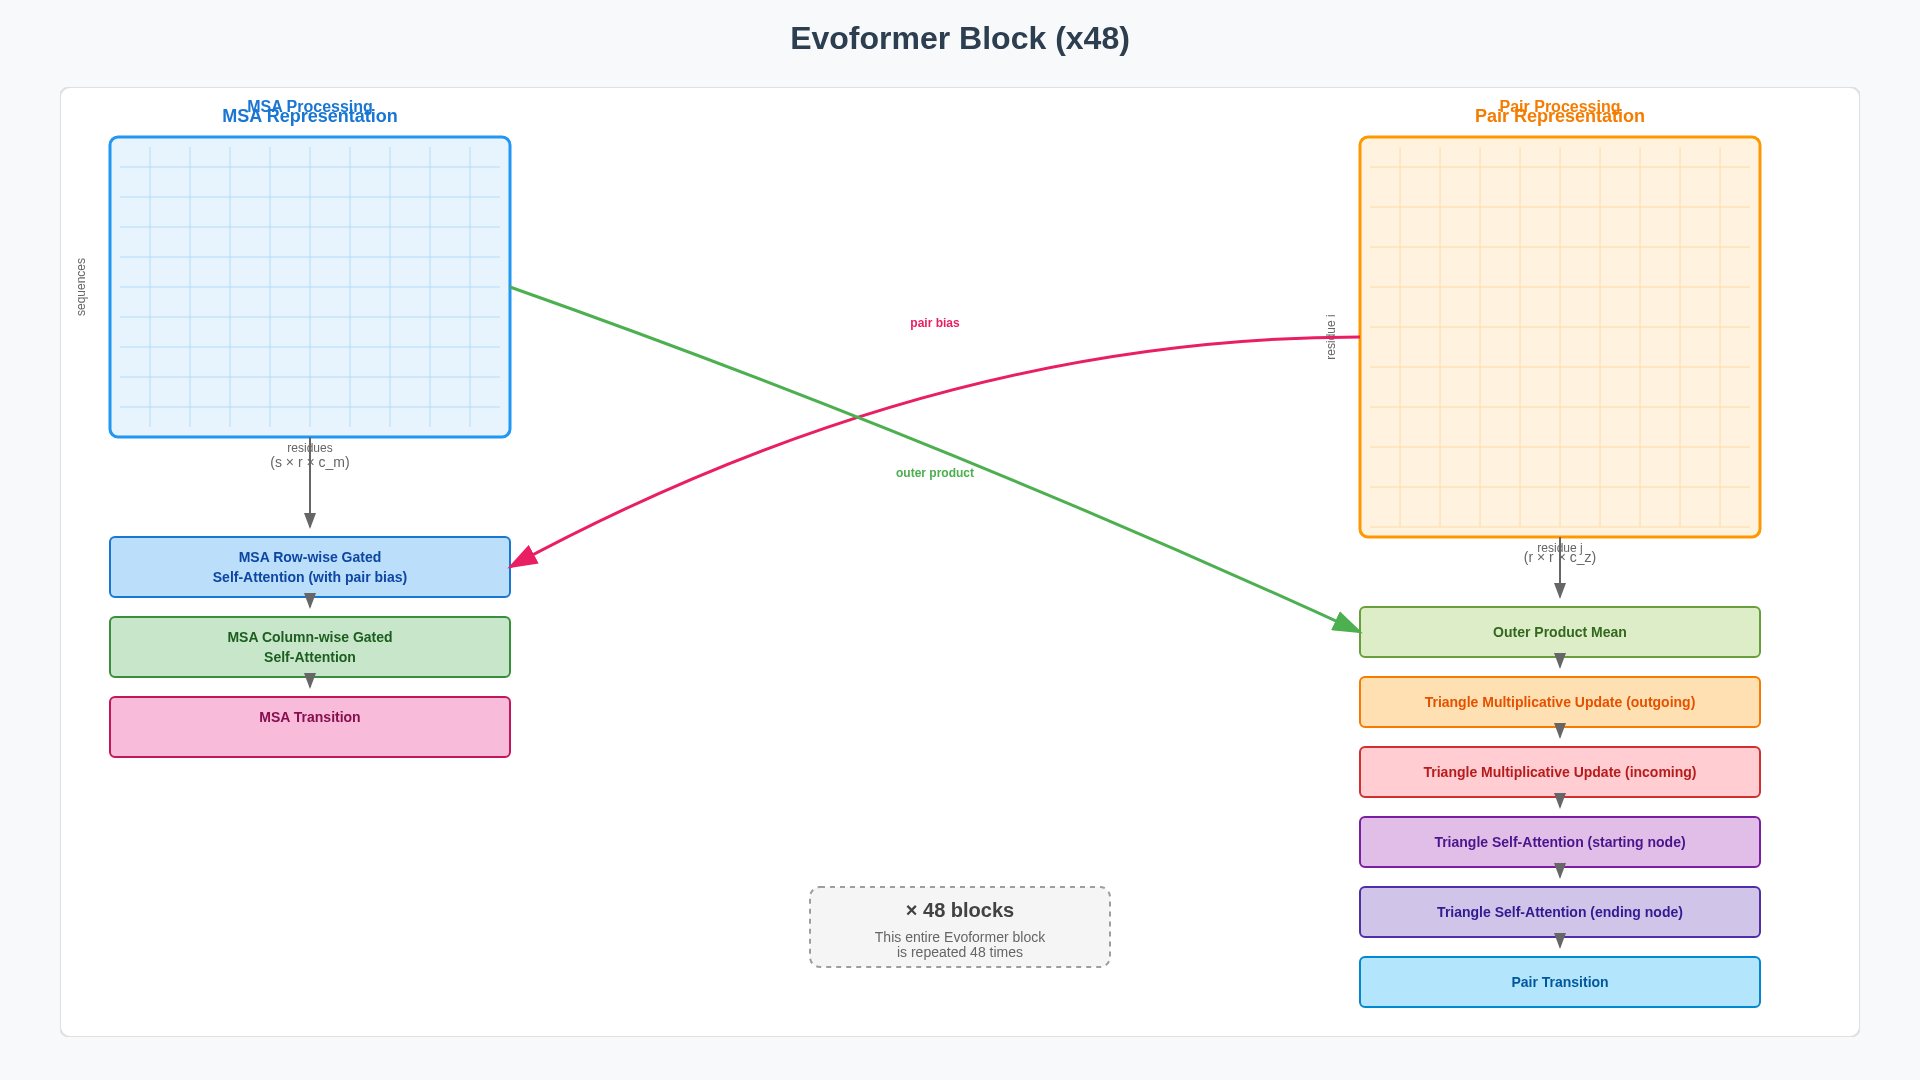
\includegraphics[width=\linewidth]{figures/evoformer_singleshot_vlm_perfect.png}
\caption{A single-shot figure the VLM rated ``perfect'': both section titles are superimposed (``MSA Processing'' over ``MSA Representation''; ``Pair Processing'' over ``Pair Representation'') and axis labels collide with the matrix borders.}
\label{fig:evoformer}
\end{subfigure}
\caption{\textbf{The default VLM judge is structurally blind to layout defects.} \textbf{(\subref{fig:blind})} On the same $15$ single-shot academic figures, the VLM-on-a-screenshot judge rates $14$ ``perfect'' while the deterministic DOM-geometry instrument finds only $3$ actually clean. The other $11$ are broken in ways cropped off-frame or below VLM acuity. \textbf{(\subref{fig:evoformer})} A representative ``perfect''-rated render whose text-on-text overlaps ($\ge6$\,px) are exactly what the geometry check flags and the screenshot judge misses.}
\label{fig:blindpair}
\end{figure}

\begin{figure}[t]
\centering
\begin{subfigure}[b]{0.49\linewidth}
\centering
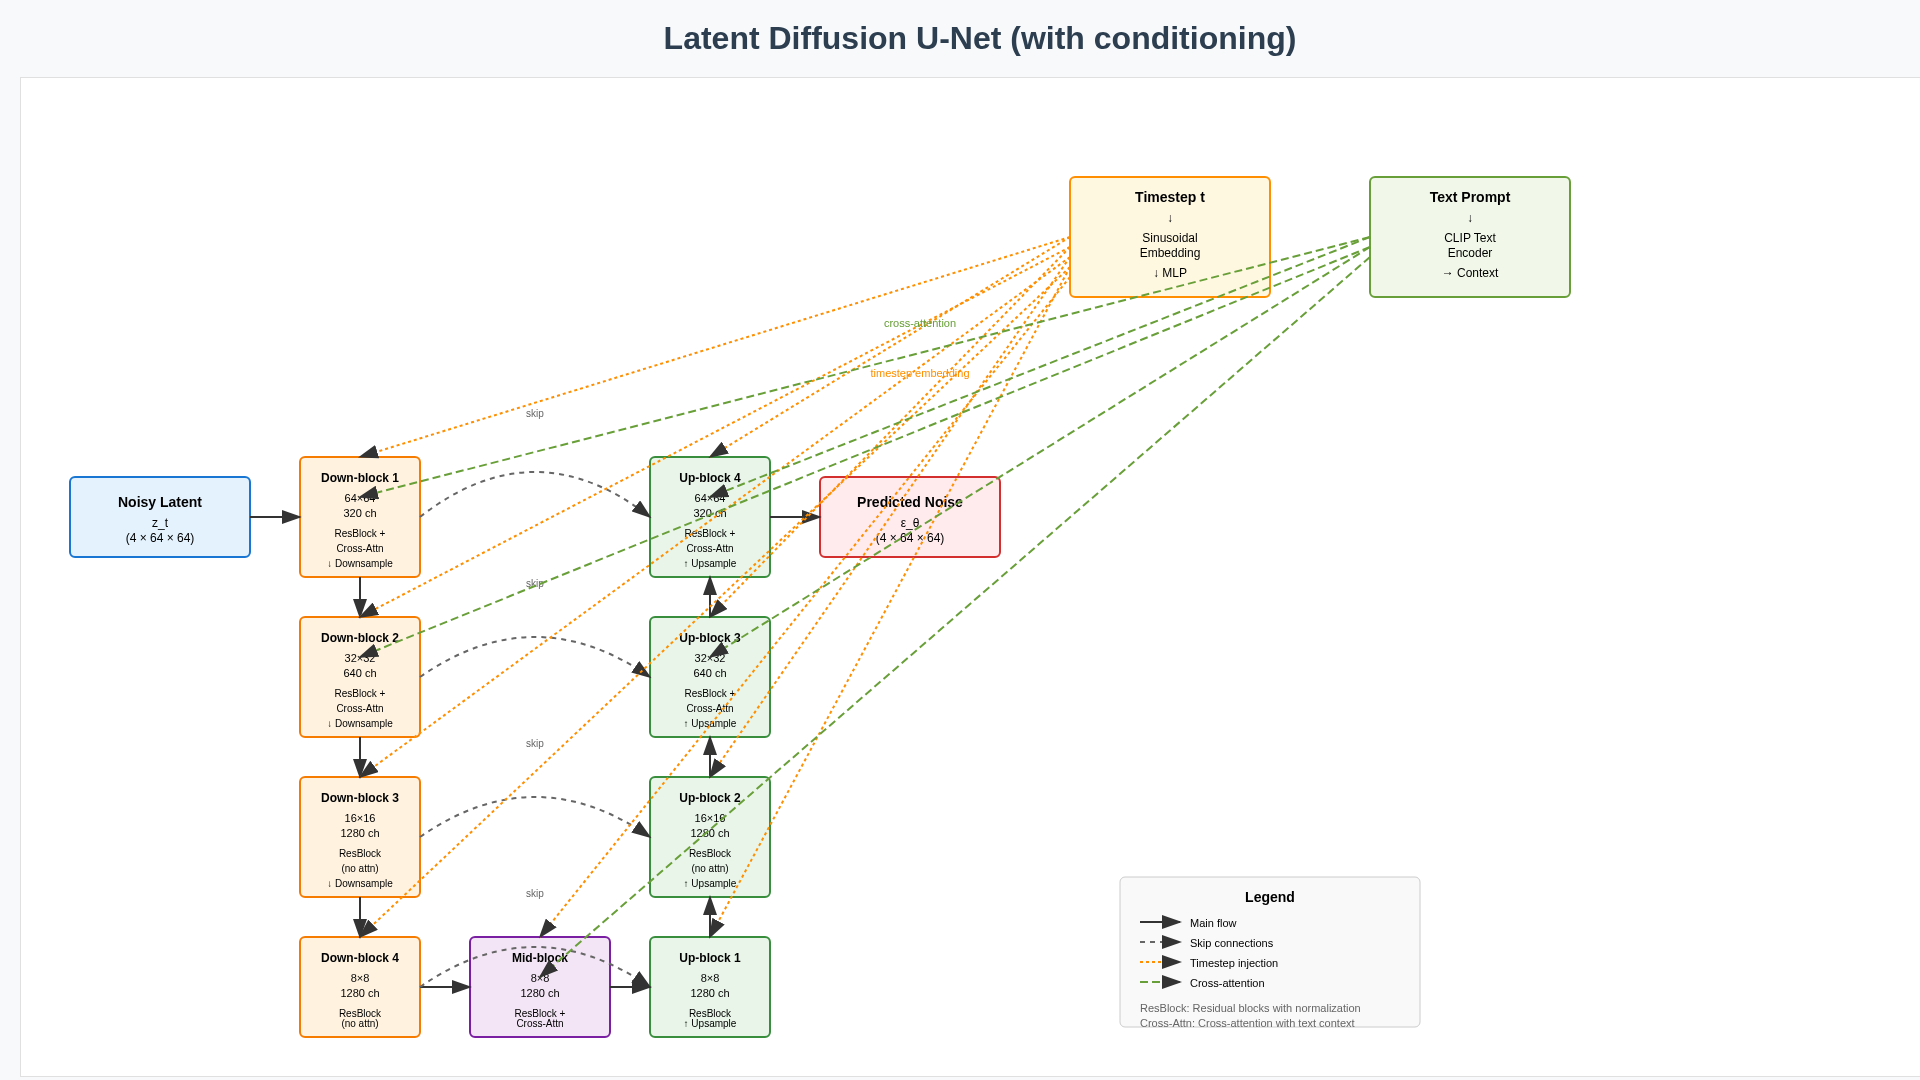
\includegraphics[width=\linewidth]{figures/diffusion_unet_singleshot.png}
\caption{\textbf{Single-shot.} Conditioning blocks crowd the down-block column, edges route through boxes and tangle at the center, and the legend collides with the decoder, all defects the geometry instrument flags but the VLM cannot see.}
\label{fig:ba-ss}
\end{subfigure}\hfill
\begin{subfigure}[b]{0.49\linewidth}
\centering
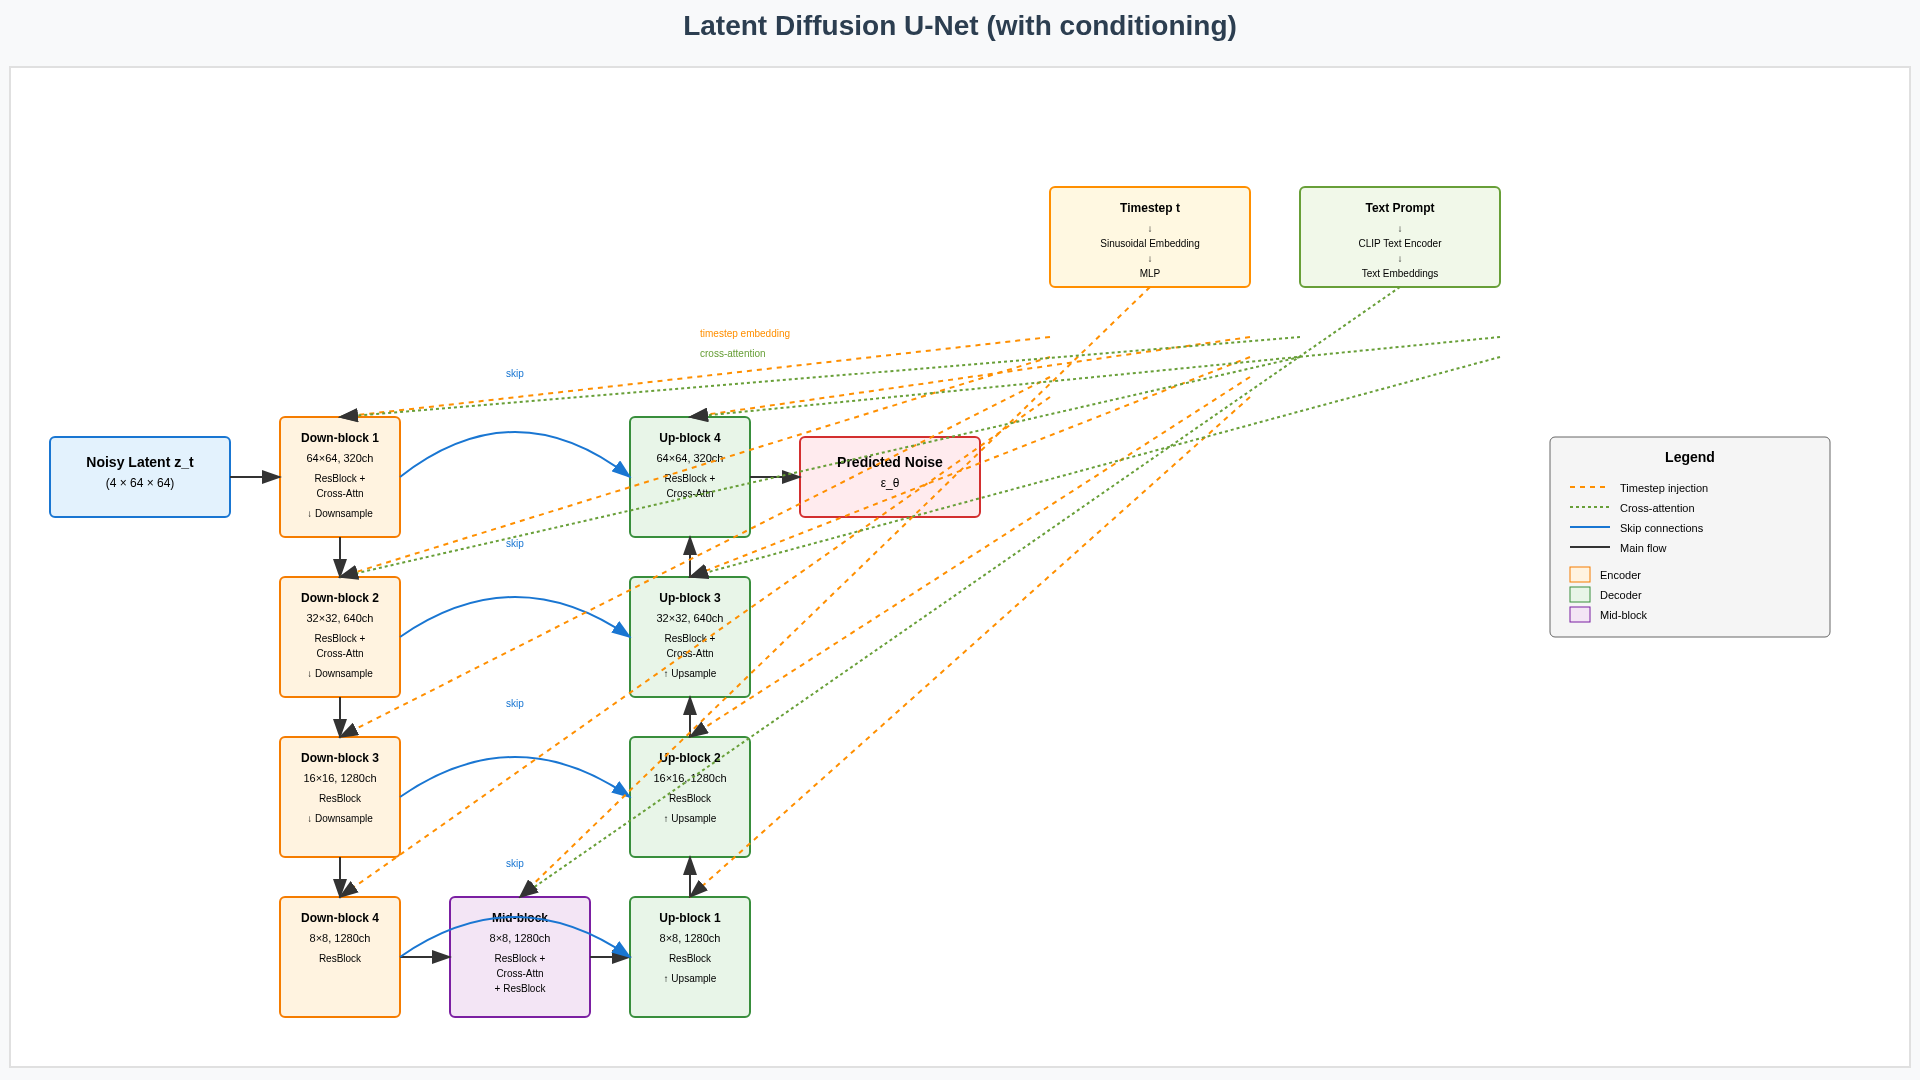
\includegraphics[width=\linewidth]{figures/diffusion_unet_reviewed.png}
\caption{\textbf{After grounded feedback.} The same task: conditioning blocks lifted clear, columns spaced and aligned, skip connections deconflicted, legend boxed in free space.}
\label{fig:ba-rv}
\end{subfigure}
\caption{\textbf{What grounded geometric feedback actually fixes.} The same academic-figure task, single-shot (\subref{fig:ba-ss}) vs.\ after the propose$\to$measure$\to$revise loop (\subref{fig:ba-rv}). This is the per-artifact reality behind the $-74\%$ mean defect reduction in \Cref{tab:geometric}, and exactly the difference a screenshot judge is blind to.}
\label{fig:beforeafter}
\end{figure}

\paragraph{A deterministic instrument reveals a large, significant effect across four modalities.} We score four visual modalities with the same DOM-geometry+alignment instrument under one identical configuration (Sonnet~4, temperature~$0$, design-principle prompt, three seeds, propose$\to$measure$\to$feed-exact-defects-back$\to$revise, $\le3$ iterations). \Cref{tab:geometric} and \Cref{fig:geomreduction} report the result: grounded geometric feedback produces a large, significant reduction in real layout defects on \emph{all four}, with bootstrap 95\% CIs that exclude zero and improvements sharply outnumbering regressions. The magnitudes track single-shot headroom: dense responsive web pages are defect-rich out of the box, while a frontier model under a design-principle prompt already lays out many figures and slides cleanly. Animations have the widest interval because their per-task defect counts are heavy-tailed across the dynamic suite, so we read the sign test as the robust statement and the mean as indicative.

\begin{table}[t]
\centering\small
\caption{Deterministic geometric-feedback results, one identical configuration across four visual modalities (Sonnet~4, $T{=}0$, $3$ seeds, alignment-inclusive reward). $\Delta$ is the mean defect reduction. CI is a paired bootstrap 95\% interval on $\Delta\%$ ($10$k resamples). $p$ is a two-sided paired sign test. Web is summed over $1920/375$ widths, animations over sampled frames.}
\label{tab:geometric}
\begin{tabular}{lcccccc}
\toprule
Modality & $n$ & SS & Rev. & $\Delta$ & 95\% CI & impr./regr.\ ($p$) \\
\midrule
Academic figures (20) & 60 & $0.57$ & $0.15$ & $-74\%$ & $[52,89]\%$ & $17/2$\;($7{\times}10^{-4}$) \\
Dense slides (12)     & 36 & $1.25$ & $0.33$ & $-73\%$ & $[45,93]\%$ & $13/1$\;($1.8{\times}10^{-3}$) \\
Web pages (20)        & 60 & $16.1$ & $8.5$  & $-47\%$ & $[30,62]\%$ & $33/2$\;($4{\times}10^{-8}$) \\
Animations (20)       & 60 & $16.9$ & $10.2$ & $-40\%$ & $[10,64]\%$ & $34/7$\;($3{\times}10^{-5}$) \\
\bottomrule
\end{tabular}
\end{table}

\begin{figure}[t]
\centering
\begin{tikzpicture}
\begin{axis}[width=0.86\linewidth,height=4.6cm,
  xbar,xmin=0,xmax=100,bar width=14pt,enlarge y limits=0.28,
  xlabel={geometric-defect reduction under grounded feedback (\%), bootstrap 95\% CI},
  symbolic y coords={Animations,Web pages,Dense slides,Academic figures},
  ytick=data,xtick={0,20,40,60,80,100},xmajorgrids]
  \addplot[draw=cRV!65!black,fill=cRV!55,
    error bars/.cd,x dir=both,x explicit,
    error bar style={cRV!60!black,line width=0.6pt},
    error mark options={cRV!60!black,mark size=2.4pt,line width=0.6pt}]
    coordinates {(74,Academic figures)+=(15,0)-=(22,0)
                 (73,Dense slides)+=(20,0)-=(28,0)
                 (47,Web pages)+=(15,0)-=(17,0)
                 (40,Animations)+=(24,0)-=(30,0)};
  % value labels at the bar base, clear of the CI whiskers
  \node[font=\footnotesize\bfseries,white,anchor=west] at (axis cs:1.8,Academic figures) {74\%};
  \node[font=\footnotesize\bfseries,white,anchor=west] at (axis cs:1.8,Dense slides) {73\%};
  \node[font=\footnotesize\bfseries,white,anchor=west] at (axis cs:1.8,Web pages) {47\%};
  \node[font=\footnotesize\bfseries,white,anchor=west] at (axis cs:1.8,Animations) {40\%};
\end{axis}
\end{tikzpicture}
\caption{\textbf{Grounded geometric feedback removes real layout defects on all four visual modalities} (mean reduction, with whiskers the paired-bootstrap 95\% CIs, all excluding zero). The standard VLM-on-a-screenshot metric measures none of this.}
\label{fig:geomreduction}
\end{figure}

\paragraph{An ungrounded \emph{reviewer} fails to fix layout, and on slides makes it worse (ablation, two modalities).} Grounding matters on the feedback side too. We fix the task suite and the proposer model and swap \emph{only} the reviewer's grounding. Because the two arms are separate runs, each is compared against its \emph{own} single-shot baseline, and single-shot geometry carries real seed-to-seed variance. So the load-bearing contrast is the \emph{direction} each reviewer moves its own baseline, not the absolute level (\Cref{fig:ablation}). The deterministic geometric-feedback reviewer sharply \emph{reduces} mean defects on both slides and figures, whereas the VLM-feedback reviewer does not: it increases defects on slides and is directionally worse on figures (not significant). Blind to the true geometry, its edits break alignment about as often as they fix it. On the same slides the binary VLM rubric simultaneously saturates, confirming the judge cannot even see the difference. Both halves of \Cref{fig:concept} are necessary.

\begin{figure}[t]
\centering
\begin{tikzpicture}
\begin{axis}[name=axslide,width=0.42\linewidth,height=3.9cm,ybar,bar width=10pt,
  ylabel={mean defects},title={\footnotesize slides},ymin=0,ymax=2.9,ytick={0,1,2},
  symbolic x coords={VLM-fb,geom-fb},xtick=data,enlarge x limits=0.6,
  nodes near coords,nodes near coords style={font=\scriptsize,/pgf/number format/.cd,fixed,precision=2},ymajorgrids]
  \addplot[draw=cGrey,fill=black!10] coordinates {(VLM-fb,1.89) (geom-fb,1.25)};
  \addplot[draw=cAccent!60!black,fill=cAccent!25] coordinates {(VLM-fb,2.44) (geom-fb,0.33)};
\end{axis}
\begin{axis}[at={($(axslide.east)+(1.4cm,0)$)},anchor=west,
  width=0.42\linewidth,height=3.9cm,ybar,bar width=10pt,
  title={\footnotesize academic figures},ymin=0,ymax=0.8,ytick={0,0.25,0.5},
  symbolic x coords={VLM-fb,geom-fb},xtick=data,enlarge x limits=0.6,
  nodes near coords,nodes near coords style={font=\scriptsize,/pgf/number format/.cd,fixed,precision=2},ymajorgrids,
  legend style={font=\footnotesize,at={(-0.14,1.26)},anchor=south,legend columns=2,draw=cGrey!50}]
  \addplot[draw=cGrey,fill=black!10] coordinates {(VLM-fb,0.52) (geom-fb,0.57)}; \addlegendentry{single-shot}
  \addplot[draw=cAccent!60!black,fill=cAccent!25] coordinates {(VLM-fb,0.62) (geom-fb,0.15)}; \addlegendentry{reviewed}
\end{axis}
\end{tikzpicture}
\caption{\textbf{An ungrounded reviewer fails to fix layout, while a grounded one does (controlled ablation, two modalities).} Same task suite and proposer model, with only the reviewer's grounding varying. The two arms are separate runs, so each is plotted against its \emph{own} single-shot (hence the differing single-shot bars). The VLM-feedback reviewer (\textsf{VLM-fb}) does not reduce defects and on slides increases them (slides $1.89\to2.44$, figures $0.52\to0.62$, directional/n.s.). The deterministic geometric-feedback reviewer (\textsf{geom-fb}) reduces them (slides $1.25\to0.33$, figures $0.57\to0.15$). The grounded signal is necessary on the feedback side, not just the metric side.}
\label{fig:ablation}
\end{figure}

\paragraph{Is the reduction circular?} The instrument both \emph{drives} the revision and \emph{scores} it, and the harness keeps the best-scoring iteration, so \emph{some} reduction is mechanically guaranteed. The honest questions are how large it is and whether it reflects quality a human would care about. Three facts argue it is not merely an artifact of optimizing the reported number. \textbf{(i)~The defects are real:} single-shot renders carry them at high rate (\Cref{fig:evoformer}), and the thresholds are deliberately conservative ($\ge6$\,px overlap, $>16$\,px overflow), so a flagged defect is visible, not sub-perceptual. \textbf{(ii)~The magnitude is not preordained:} keeping the best of three iterations could in principle move the metric by almost nothing. That grounded revision instead removes a large fraction of real defects (\Cref{tab:geometric}) is a property of the feedback, not the keep-best rule. \textbf{(iii)~The ungrounded-reviewer ablation is the decisive control:} scored by the \emph{same} metric, the VLM-feedback arm \emph{fails} to reduce it (and worsens slides). So the reduction tracks the \emph{grounding} of the feedback, not the act of optimizing the scorer, a conclusion the model-free cross-model replication (\Cref{sec:robustness}) reinforces. What remains open, and is the principal caveat of the geometric measurement, is a quantitative human-preference study confirming that DOM-defect reduction maps onto perceived-quality gains across the full suite.

\paragraph{Two modalities where the honest answer is ``no headroom.''} \emph{Video editing}, scored by Gemini~3.1~Pro's native full-clip rubric (a near-grounded instrument that observes pixels, not a still), is already strong single-shot, so the reviewed lift is small and not significant. A hardened multi-step suite de-saturates it. \emph{Deep research}, scored against exact provided facts, saturates: a frontier model knows well-documented facts and does not take the planted traps, so the Type-3d lift is bounded by the near-zero single-shot error rate. This is a genuine limit of the factual modality, since de-saturating it would require facts the judge itself cannot grade. We report these as scoped negatives rather than headline lifts (\Cref{tab:harness-headline}).

\section{Robustness}
\label{sec:robustness}

\paragraph{Cross-model, code.} The effect is architectural, not a Claude artifact. On the $15$ hard code tasks the harness lifts Sonnet~4 by $+33.3$\,pp (to $100\%$), Qwen3-235B by $+26.7$\,pp, and GPT-5 by $+13.3$\,pp (on a higher single-shot baseline). All three families benefit from the same execution-grounded loop.

\paragraph{Cross-model, grounded geometry.} To rule out a Claude-specific or prompt-specific explanation of the grounded-evaluation effect, we run the same deterministic geometric-feedback harness with \textbf{Gemini~3.1~Pro} as the proposer on the dense responsive-web suite, scored by the identical model-free DOM instrument. Because the instrument depends on no model, a reduction here is attributable to the grounded loop rather than to the scorer; it reproduces the direction of \Cref{tab:geometric} on a different model family.

\paragraph{Held-out generalization.} On a $32$-task held-out code suite constructed after the method was fixed, the harness lifts $90.6\%\to100\%$, recovering $3/3$ first-shot failures with zero regressions---no tuning to the original tasks.

\paragraph{Budget allocation.} Sweeping the proposer/reviewer token split on a fixed budget produces an $86.6$\,pp spread in pass-rate, monotone in the proposer's per-call share: the optimum is \emph{propose-heavy} (allocate the majority to generation, reserve enough for the reviewer to localize defects). Extra inference compute is better spent on additional samples than on deeper iteration past the early-stop point.

\section{Internalizing the Harness into a Small Student}
\label{sec:distill}

Two things could carry the harness's gains: the grounded scaffolding, or behavior absorbed into the weights. This section asks how much is the latter---whether the loop's interaction quality can be \emph{internalized} so a small model emits high-quality artifacts in fewer passes. It is a complement to the thesis, not a substitute: the cheaper internalized proposer is still meant to run \emph{inside} the same grounded harness, so internalization and grounding compose. We distill judge-filtered teacher trajectories from the harness into an $8$B Qwen3-VL student via supervised fine-tuning.

\paragraph{Result.} The student recovers about half the teacher's single-sample capability on an out-of-distribution suite, and a second sample closes much of the remaining gap (\Cref{fig:distill})---at roughly $10\times$ lower deployment cost than running the harness over a frontier model. On a harder held-out suite of the teacher's own pre-curated failures it passes a substantial fraction (\Cref{tab:distill-headline}), and run back inside the harness it recovers still more.

\begin{figure}[t]
\centering
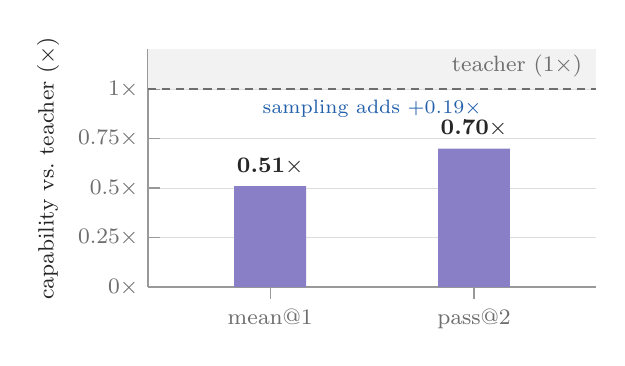
\begin{tikzpicture}
\begin{axis}[paperbar,width=0.6\linewidth,height=4.6cm,clip=false,
  ybar,bar width=26pt,ymin=0,ymax=1.2,
  ylabel={capability vs.\ teacher ($\times$)},
  symbolic x coords={mean@1,pass@2},xtick=data,enlarge x limits=0.6,
  x tick label style={font=\footnotesize,color=cMut},
  ymajorgrids,ytick={0,0.25,0.5,0.75,1.0},yticklabel={\pgfmathprintnumber{\tick}$\times$}]
  % teacher reference band spanning the full plot width
  \fill[black!5] ({rel axis cs:0,0}|-{axis cs:mean@1,1.0}) rectangle ({rel axis cs:1,0}|-{axis cs:mean@1,1.2});
  \draw[cMut,densely dashed,line width=0.7pt] ({rel axis cs:0,0}|-{axis cs:mean@1,1.0}) -- ({rel axis cs:1,0}|-{axis cs:mean@1,1.0});
  \node[font=\footnotesize,cMut,anchor=south east] at ({rel axis cs:0.99,0}|-{axis cs:mean@1,1.01}) {teacher ($1\times$)};
  \addplot[draw=none,fill=cStu!65] coordinates {(mean@1,0.51) (pass@2,0.70)};
  \node[font=\footnotesize\bfseries,cInk,anchor=south] at (axis cs:mean@1,0.52) {0.51$\times$};
  \node[font=\footnotesize\bfseries,cInk,anchor=south] at (axis cs:pass@2,0.71) {0.70$\times$};
  \node[font=\scriptsize,cGnd!80!black,anchor=center]
    at ($(axis cs:mean@1,0.90)!0.5!(axis cs:pass@2,0.90)$)
    {sampling adds $+0.19\times$};
\end{axis}
\end{tikzpicture}
\caption{\textbf{An $8$B student internalizes much of the teacher's interaction quality.} Distilled student as a fraction of the frontier teacher on the $44$-task out-of-distribution suite (\Cref{tab:distill-ood}): one sample recovers $0.51\times$ and two samples $0.70\times$ of teacher capability, at ${\sim}10\times$ lower deployment cost. On the $18$-task hard held-out suite the same student passes $44\%$ at pass@$1$ and $56\%$ at pass@$3$ (\Cref{tab:distill-headline}).}
\label{fig:distill}
\end{figure}

\paragraph{Variance is a budget (a cautionary finding).} Reinforcement fine-tuning (RFT) on top of SFT improves every per-turn consistency metric we measure \emph{and} regresses pass@$k$ (\Cref{fig:variance}). The two students start nearly tied on a single sample; as samples are added, the SFT student keeps converting draws into new solved tasks while the RFT student's curve goes flat. The reading is that for sampling-based deployment, output-distribution variance \emph{is} the inference-scaling lever, and any post-training that reduces it spends from the same budget best-of-$N$ draws on. Variance is not noise to minimize; it is the resource sampling converts into quality. The operational recipe is therefore: SFT to internalize interaction quality, keep the proposer's sampling temperature, and run it inside the grounded harness.

\begin{figure}[t]
\centering
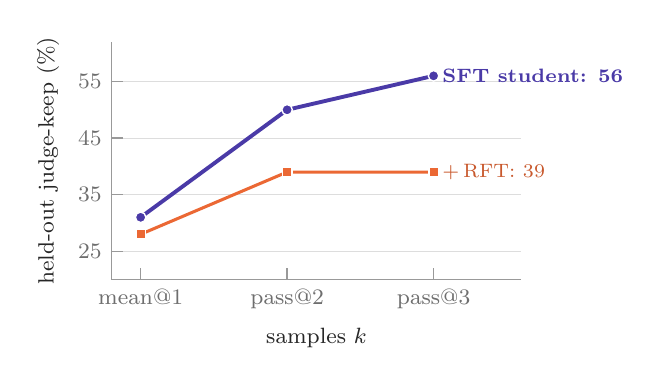
\begin{tikzpicture}
\begin{axis}[width=0.56\linewidth,height=4.6cm,
  xlabel={samples $k$},ylabel={held-out judge-keep (\%)},
  xmin=0.8,xmax=3.6,ymin=20,ymax=62,clip=false,
  xtick={1,2,3},xticklabels={mean@1,pass@2,pass@3},
  x tick label style={font=\footnotesize,color=cMut},
  ytick={25,35,45,55},ymajorgrids,
  axis x line*=bottom,axis y line*=left]
  \addplot[cStu,line width=1.4pt,mark=*,mark size=1.9,
    mark options={fill=cStu,draw=white,line width=0.5pt}]
    coordinates {(1,31)(2,50)(3,56)};
  \addplot[cUng,line width=1.1pt,mark=square*,mark size=1.7,
    mark options={fill=cUng,draw=white,line width=0.5pt}]
    coordinates {(1,28)(2,39)(3,39)};
  \node[font=\scriptsize\bfseries,cStu,anchor=west,inner sep=3pt] at (axis cs:3,56) {SFT student: 56};
  \node[font=\scriptsize,cUng!85!black,anchor=west,inner sep=3pt] at (axis cs:3,39) {+\,RFT: 39};
\end{axis}
\end{tikzpicture}
\caption{\textbf{RFT polishes consistency but spends the variance that sampling needs.} Judge-keep vs.\ number of samples on the $18$-task hard held-out suite for the chosen SFT student and the same student after RFT. RFT improves every per-turn consistency metric (\Cref{tab:distill-rft}) yet regresses pass@$3$ by $17$\,pp: the near-tie at one sample and the flat curve past it show the lost quality is exactly the distributional spread best-of-$N$ converts into solved tasks.}
\label{fig:variance}
\end{figure}

\section{Related Work}
\label{sec:related}

\paragraph{Test-time compute scaling.} Two axes are established. \emph{Reasoning} scaling (chain-of-thought, tree search, and extended thinking \citep{wei2022chain,yao2023tree,deepseek2025r1,snell2024scaling,kimi2025k15}) spends more tokens before committing. \emph{Sampling} scaling (self-consistency and best-of-$N$ \citep{wang2023selfconsistency,brown2024large}) draws multiple attempts and selects one. Both only rework the same frozen weights and prompt (both are \emph{internal} in the sense of \Cref{sec:framework}, which makes precise how they are bounded). We position \emph{interaction} as a third, external axis that imports information the model does not have.

\paragraph{Self-correction and critique.} Iterative refinement with model-generated feedback (Reflexion \citep{shinn2023reflexion}, ReAct \citep{yao2023react}, Self-Refine \citep{madaan2023selfrefine}, CRITIC \citep{gou2024critic}) is widely used, but its reliability is contested: \citet{huang2024selfcorrect} show that models often cannot self-correct reasoning without an external signal, and \citet{kamoi2025correct} chart when correction does and does not help. Our taxonomy makes the distinction explicit: \emph{ungrounded} critique is subject to the internal ceiling, while refinement against an executed or measured observation is not. Our controls (\Cref{sec:feedback}) then show that it is the instrument's coverage of the defect, not the extra critique pass, that carries the gain.

\paragraph{Grounded and execution feedback.} Tool use and execution feedback (Toolformer \citep{schick2023toolformer}, Gorilla \citep{patil2024gorilla}, Voyager \citep{wang2023voyager}, RLEF \citep{gehring2025rlef}, and, for website generation specifically, WebGen-Agent's multi-level visual/functional feedback \citep{webgen2025}), together with the thinking-vs-doing analysis of \citet{shen2025thinking}, establish that acting on an environment helps. We contribute the information account of \emph{why}, a coverage principle that predicts \emph{when}, and, crucially, the requirement that the \emph{evaluation} be grounded too. We also compare harness architectures (single-agent loops \citep{trankiela2026singleagent}, sample-and-select \citep{ruan2025iad}, proposer--reviewer) under a matched budget.

\paragraph{Model-as-judge reliability.} LLM- and VLM-as-judge evaluation is now standard \citep{zheng2023judging}, and its failure modes (position, verbosity, and self-preference biases, and broader reward-model fragility \citep{casper2023open}) are documented. Our finding is sharper and, to our knowledge, not previously isolated: for artifacts whose quality is a measurable \emph{physical} property (the geometry of a rendered layout), a screenshot judge is not merely biased but \emph{structurally blind} (the defect is dropped by its observation channel before judgment begins), so it both fails to score the defect and, used as a reviewer, fails to fix it. This is why a deterministic instrument is necessary, not merely preferable, to detect interaction scaling on visual modalities.

\paragraph{Practitioner evidence at scale.} Industrial deployment corroborates the gap our framework targets. \citet{hong2026aicoding} reports a controlled study at ByteDance ($3$ frontier coding models $\times$ $3$ agent frameworks $\times$ $100$ runs) on a single real product feature: functional \emph{correctness} exceeded $80\%$ for every pair, yet ``deliverability'' axes (usability, reliability, maintainability, performance) collapsed to $40$--$60\%$ and rose to ${\sim}80\%$ only after harness ``infrastructure'' was added, while correctness barely moved. This is the signature we formalize: internal scaling saturates the easy-to-see axis while the interaction loop carries the rest. Tellingly, the report had to define a multi-axis quality metric before the gap was visible at all (an industrial analogue of our grounded-evaluation requirement), and its grounded fixes (e.g.\ browser-driven validation before commit) are instrument observations in our taxonomy, not ungrounded self-review.

\paragraph{Information theory.} The data-processing inequality \citep{cover2006elements} underlies the formal version of the internal ceiling (\Cref{app:ceiling}): any post-processing of the model's outputs (reasoning, ungrounded review) cannot increase information about the target, whereas an instrument observation introduces a new channel.

\section{Discussion and Conclusion}
\label{sec:discussion}

\paragraph{Grounding is the load-bearing variable.} Two of the three test-time axes are bounded by the data-processing inequality because they never leave the model's token space; the third is unbounded precisely because grounded feedback imports external information each cycle. We have argued and shown that this grounding must hold on \emph{both} sides of the loop. On the feedback side, an in-modality control isolates test \emph{execution}---not the extra review pass---as the active ingredient, and a VLM \emph{reviewer} of slide layout actively regresses quality. On the evaluation side, the default VLM-on-a-screenshot metric is structurally blind to the geometric defects the loop fixes, so the entire visual-modality effect is invisible until the metric is grounded in deterministic DOM geometry---at which point grounded feedback removes $40$--$74\%$ of real layout defects across four modalities, every CI excluding zero.

\paragraph{A methodological warning for the field.} Much of the recent excitement about ``LLMs that critique and improve their own visual output'' is measured with VLM judges. Our results imply many such measurements are uninformative on layout: the judge cannot see the defects, and using it as the reviewer can make things worse. Where an artifact's quality is a measurable physical property---geometry, execution, retrieval---the evaluation should be grounded in that property, not in a model's picture of it.

\paragraph{Limits, honestly stated.} Two modalities saturate: video editing is already strong single-shot (the lift is real only on a hardened multi-step suite), and deep research saturates because frontier models know well-documented facts and the judge cannot grade facts they do not. Deterministic geometry applies to artifacts with a measurable intended layout (figures, slides, web, animations); for genuinely flowing content we still rely on a binary rubric, with the VLM-reliability caveat.

\paragraph{Future work and broader impact.} Two directions follow directly. First, deterministic instruments for modalities beyond layout and execution---differentiable or symbolic checks for audio, 3D, tabular, and UI-interaction artifacts---would extend grounded evaluation to where VLM/LLM judges are likewise blind. Second, our DPI argument bounds an information channel; tightening it into a quantitative relationship between feedback fidelity and achievable quality is open. On impact: grounding the metric is a cheap, deployable correction to a measurement error that, we argue, currently inflates reported progress on self-improving visual generation; the same instruments are auditable and reduce reliance on opaque model judges. The harness itself is scaffolding over a frozen model, so it inherits that model's capabilities and failure modes rather than introducing new ones.

\paragraph{Operational recipe.} Wrap a frozen frontier model in a proposer--reviewer harness with the most actionable grounded feedback channel for the modality. For visual artifacts, ground \emph{both} the reviewer and the scorer in deterministic geometry---measure the rendered DOM, never a screenshot. Allocate the majority of the per-task budget to the proposer; spend extra compute on samples, not deeper iteration. For cost-sensitive deployment, distill the proposer into a small student and run it inside the same harness. Interaction scaling is real, distinct from reasoning and sampling, predictable from the feedback taxonomy, and---once you ground the metric---plainly visible.


\section*{Acknowledgements}

This paper was produced using Pine Copilot's voice-directed \emph{whisper coding} workflow~\citep{pineai2026whispercoding}, in which the authors specify, discuss, and review the work by voice while a coding agent---Claude Code with Claude Opus 4.8---carries out the planning, coding, experiments, and paper writing.
We thank BSQL Networking for hosting the NVIDIA RTX PRO 6000 GPU.

\bibliographystyle{plainnat}
\bibliography{refs}

\appendix
\section{Detailed Results and Configurations}
\label{app:detailed}
This appendix collects the full tables underlying the summaries in the main text: the four-strategy scaling curves, the matched-budget reasoning baseline, the in-modality feedback-type control, the single-agent-vs-harness comparison, cross-model and held-out code, the budget-allocation simplex, token ROI by modality, the distillation ablations, the per-task pass@$k$ breakdown for the $8$B student, and the original six-modality holistic overview (superseded for the visual modalities by the grounded measurements of \Cref{sec:grounded_eval}).

\subsection{Four-strategy scaling at a matched 20K-token budget}
\begin{table}[t]
\centering
\caption{\textbf{The headline scaling result (3-seed mean $\pm$ SD).} Pass-rate by strategy~$\times$~budget on 15 hard code tasks, Sonnet 4. S, L, and H are averaged over three independent on-policy runs; R was run once (extended-thinking variation across seeds is small at temp~0) at the sweep's budget partition (a more generous partition lifts R to $86.7\%$; see footnote and \Cref{tab:reasoning-baseline}). S's small dip from $B{=}1$K (80.0\%) to $B{=}5$K (77.8\%) is within the $\pm 3.1$\,pp seed noise on a 3-seed $\times$ 15-task suite; pass@$N$ is non-decreasing in $N$ in expectation but not pointwise across finite-sample on-policy seeds. \emph{Reasoning-only and best-of-$N$ saturate well below 100\%}; all three iteration-with-feedback strategies reach $\geq97.8\%$ at $B{=}20$K (L hit 100\% on 2 of 3 seeds; H on all 3; H is the only variant at strict 100\% across seeds). The architectural ordering across H, L is within seed noise on pass-rate; what separates them is token efficiency and reliability (\Cref{sec:interaction}).}
\label{tab:scaling-curves}
\small
\begin{tabular}{lcccc}
\toprule
Budget $B$ & R (reasoning-only) & S (best-of-$N$) & L (single-agent loop) & H (proposer--reviewer) \\
\midrule
1K   & 60.0\% & 80.0\% $\pm 0.0$\,pp & 57.8\% $\pm 3.1$\,pp & 62.2\% $\pm 3.1$\,pp \\
5K   & 73.3\% & 77.8\% $\pm 3.1$\,pp & \textbf{93.3\% $\pm 0.0$\,pp} & 91.1\% $\pm 3.1$\,pp \\
20K  & 73.3\% & 86.7\% $\pm 0.0$\,pp & 97.8\% $\pm 3.1$\,pp & \textbf{100.0\% $\pm 0.0$\,pp} \\
\midrule
Ceiling & 73.3\% & 86.7\% & $\sim$100\% & \textbf{100\% (zero variance)} \\
\bottomrule
\end{tabular}
\end{table}

\subsection{Reasoning-only at a matched budget}
\begin{table}[ht]
\centering
\caption{Reasoning-only at matched budget vs.\ single-shot and the harness on the 15 hard code tasks. Single-seed numbers (the Phase-1 reference seed, also used in \Cref{tab:type-controls}); the 3-run aggregate is reported in \Cref{tab:harness-headline} ($66.7 \pm 6.7$\% single-shot, $100.0 \pm 0.0$\% reviewed). Reasoning closes two-thirds of the harness's gap over single-shot but falls 6.7\,pp short of the harness's pass-rate even at $1.57\times$ the harness's token budget.}
\label{tab:reasoning-baseline}
\small
\begin{tabular}{lccc}
\toprule
Strategy & Pass-rate & Mean tokens & $\Delta$ vs.\ single-shot \\
\midrule
Single-shot                       & 73.3\% (11/15) & 1{,}406  & --- \\
Reasoning-only (matched budget)   & 86.7\% (13/15) & 4{,}137  & $+13.3$\,pp \\
\textbf{Proposer--reviewer harness} & \textbf{93.3\% (14/15)} & \textbf{2{,}643}  & $\mathbf{+20.0}$\,pp \\
\bottomrule
\end{tabular}
\end{table}

\subsection{In-modality feedback-type control (Type 1/2/3a) on a fixed code suite}
\begin{table}[ht]
\centering
\caption{In-modality feedback-type controls on 15 hard code tasks (Sonnet 4 proposer and reviewer). Each row is a single on-policy seed; the ``SS'' column is the \emph{per-seed} single-shot pass-rate (not held constant across rows) and ``Reviewed'' is the ceiling after that seed's harness run. The three SS values (10/15 and 11/15) are draws from the same single-shot distribution that gives \Cref{tab:harness-headline}'s 3-run mean of $66.7 \pm 6.7$\% (i.e.\ within the $\pm 1$\,SD band centered on 10/15). Because the SS column varies by row, the load-bearing comparison is the \emph{reviewed} ceiling: Type 3a reaches 14/15, Type 1/2 reach 13/15 ($+6.7$\,pp), \emph{and} Type 3a is $\sim$2.5$\times$ more token-efficient (1.53 vs.\ 2.07 iterations).}
\label{tab:type-controls}
\small
\begin{tabular}{lcccc}
\toprule
Type & Reviewer sees & SS & Reviewed & Iters \\
\midrule
None (single-shot)             & ---                                  & 11/15 & ---            & --- \\
Type 1 (cross-review)          & code only                            & 10/15 & 13/15          & 2.07 \\
Type 2 ($+$\texttt{ruff})      & code $+$ static analysis             & 11/15 & 13/15          & 2.07 \\
\textbf{Type 3a ($+$exec)}     & code $+$ test stderr/traceback       & 11/15 & \textbf{14/15} & \textbf{1.53} \\
\bottomrule
\end{tabular}
\end{table}

\subsection{Single-agent loop vs.\ proposer--reviewer harness}
\begin{table}[ht]
\centering
\caption{Three interaction-strategy variants at $B{=}20$K on the 15 hard code tasks, all using Type 3a execution feedback. Pass-rate is within seed noise (sign-test $p{>}0.6$ on the H--L comparison); the harness wins on \emph{token efficiency} (1{,}029 vs.\ 1{,}431 L vs.\ 1{,}416 IAD mean output tokens) and on \emph{seed variance} (zero across three seeds for H; L hit 100\% in 2 of 3 seeds; IAD was run for one seed only).}
\label{tab:LvsH}
\small
\begin{tabular}{lccc}
\toprule
Strategy & Pass-rate & Mean tokens & Notes \\
\midrule
L (single-agent loop)              & 97.8\% $\pm 3.1$\,pp (3 seeds)           & 1{,}431          & 1 task in 1 seed \\
IAD (oracle, K=3, T=0.7)           & 100.0\% (1 seed)                         & 1{,}416          & $+38$\% tokens vs.\ H \\
\textbf{H (proposer--reviewer)}    & \textbf{100.0\% $\pm 0.0$\,pp (3 seeds)} & \textbf{1{,}029} & zero seed variance \\
\bottomrule
\end{tabular}
\end{table}

\subsection{Cross-model replication (code)}
\begin{table}[ht]
\centering
\caption{Cross-model replication on the same 15 hard code tasks. The Claude row is the multi-run reference from \Cref{tab:harness-headline}; Qwen and GPT-5 are single on-policy runs at $T{=}0.7$. The harness lift survives across three families (Anthropic, Alibaba, OpenAI).}
\label{tab:crossmodel}
\small
\begin{tabular}{lccc}
\toprule
Model & Single-shot pass & Reviewed pass & $\Delta$ (lift) \\
\midrule
Claude Sonnet 4 (3-run mean)        & $66.7 \pm 6.7$\%   & $\mathbf{100.0 \pm 0.0}$\%      & $\mathbf{+33.3}$\,pp \\
Qwen3-235B-Instruct-2507 (1 run)    & $66.7$\% (10/15)   & $\mathbf{93.3}$\% (14/15)       & $\mathbf{+26.7}$\,pp \\
GPT-5 (1 run)                       & $86.7$\% (13/15)   & $\mathbf{100.0}$\% (15/15)      & $\mathbf{+13.3}$\,pp \\
\bottomrule
\end{tabular}
\end{table}

\subsection{Held-out generalization (code)}
\begin{table}[ht]
\centering
\caption{Held-out generalization on 32 newly constructed code tasks (zero overlap with the 15-task development set). The harness recovers 3/3 single-shot failures and regresses zero passing tasks. The smaller absolute $\Delta$ is a baseline-compression effect (single-shot is 90.6\% on the held-out set, leaving at most 9.4\,pp headroom).}
\label{tab:heldout}
\small
\begin{tabular}{lccccc}
\toprule
Split & $N$ & Single-shot & Reviewed & $\Delta$ & SS-fail fixes / regressions \\
\midrule
Development (3-run mean) & 15 & $66.7 \pm 6.7$\% & $100.0 \pm 0.0$\% & $+33.3$\,pp & 5/5 / 0 \\
\textbf{Held-out v2}     & 32 & $90.6$\% & $\mathbf{100.0}$\% & $\mathbf{+9.4}$\,pp & $\mathbf{3/3}$ / $\mathbf{0}$ \\
\bottomrule
\end{tabular}
\end{table}

\subsection{Budget-allocation simplex}
\begin{table}[ht]
\centering
\caption{Budget allocation simplex on 15 hard code tasks, $B = 10$K total. Pass-rate is monotone in the proposer's per-call cap; review-heavy corners (low $b_1$) collapse. The 9-point sweep yields an 86.6\,pp spread.}
\label{tab:allocation}
\small
\begin{tabular}{lccccc}
\toprule
Allocation & $b_1$ (prop) & $b_2$ (exec) & $b_3$ (rev) & Pass-rate & Mean tokens \\
\midrule
\textbf{A (propose-heavy)} & 0.80 & 0.10 & 0.10 & \textbf{93.3\% (14/15)} & 3{,}101 \\
\textbf{G (prop-dominant)} & 0.50 & 0.25 & 0.25 & \textbf{93.3\% (14/15)} & 2{,}697 \\
D (prop+exec)              & 0.40 & 0.40 & 0.20 & 80.0\% (12/15) & 4{,}025 \\
E (prop+review)            & 0.40 & 0.20 & 0.40 & 80.0\% (12/15) & 4{,}388 \\
I (equal)                  & 0.33 & 0.34 & 0.33 & 66.7\% (10/15) & 4{,}845 \\
H (review-dominant)        & 0.25 & 0.25 & 0.50 & 40.0\% (6/15)  & 7{,}485 \\
F (exec+review)            & 0.20 & 0.40 & 0.40 & 13.3\% (2/15)  & 8{,}771 \\
B (execute-heavy)          & 0.10 & 0.80 & 0.10 & \phantom{0}6.7\% (1/15)  & 9{,}383 \\
C (review-heavy)           & 0.10 & 0.10 & 0.80 & \phantom{0}6.7\% (1/15)  & 9{,}383 \\
\midrule
\multicolumn{4}{r}{Spread:} & \textbf{86.6\,pp} & \\
\bottomrule
\end{tabular}
\end{table}

\subsection{Token ROI by modality}
\begin{table}[ht]
\centering
\caption{Per-task token cost and quality return-on-investment for the harness, averaged across three on-policy runs. ``Extra tokens'' is reviewed-minus-single-shot per task. Tokens per 0.01 quality is extra tokens divided by (mean reviewed quality $-$ mean single-shot quality)$\cdot 100$. Code dominates by $100\times$.}
\label{tab:harness-roi}
\small
\begin{tabular}{lrrrr}
\toprule
Modality & Single-shot tokens & Reviewed tokens & Extra tokens & Tokens / 0.01 quality \\
\midrule
Code        & 3{,}336  & 4{,}575  & 1{,}239  & \textbf{37} \\
Video       & 3{,}808  & 20{,}584 & 16{,}776 & 359 \\
Research    & 14{,}116 & 27{,}793 & 13{,}677 & 2{,}415 \\
Webpages    & 14{,}060 & 80{,}148 & 66{,}088 & 5{,}128 \\
Animations  & 25{,}491 & 89{,}009 & 63{,}518 & 4{,}331 \\
Slides      & 10{,}274 & 36{,}956 & 26{,}682 & 4{,}447 \\
\bottomrule
\end{tabular}
\end{table}

\subsection{Distillation: headline}
\begin{table}[ht]
\centering
\caption{Distilled 8B student on the 18-task hard held-out suite (teacher's pre-curated single-shot failures, so teacher single-shot is 0/18 by construction). The student lifts judge-keep from 0\% to 44\% at pass@1 and 56\% at pass@3. The $0.50\times$ capability ratio against the teacher is established on a separate 44-task out-of-distribution suite reported next, where teacher single-shot is non-degenerate.}
\label{tab:distill-headline}
\small
\begin{tabular}{lcc}
\toprule
Setup & Compute & Judge-keep \\
\midrule
1 sample $\times$ 5 turns                                  & $1\times$ & 44\% (8/18) \\
1 sample $\times$ 8 turns                                  & $1.6\times$ & 28\% (regressed) \\
\textbf{3 samples $\times$ 5 turns (pass@3)}               & $3\times$ & \textbf{56\% (10/18)} \\
\bottomrule
\end{tabular}
\end{table}

\subsection{Distillation: capability U-curve over force-close budget}
\begin{table}[ht]
\centering
\caption{Reasoning-cap U-curve on the 18-task hard held-out suite. SFT recipe sweep on Qwen3-VL-8B-Instruct (37 judge-kept teacher traces; same inference protocol). The optimum is at the student's coherence horizon, not the teacher's.}
\label{tab:distill-ucurve}
\begin{tabular}{lccc}
\toprule
Variant & Reasoning cap (chars) & Judge-keep & Identical-retry \\
\midrule
V1 (no reasoning)     & 0    & 6\%  & 67\% \\
V4                    & 1000 & 11\% & 35\% \\
V2                    & 3000 & 17\% & 32\% \\
\textbf{V3 (chosen)}  & \textbf{1500} & \textbf{44\%} & 10\% \\
\bottomrule
\end{tabular}
\end{table}

\subsection{Distillation: data-scale}
\begin{table}[ht]
\centering
\caption{Three independent attempts to scale the SFT corpus past V3's 37 examples. All regressed. Quality dominates quantity at this scale.}
\label{tab:distill-datascale}
\begin{tabular}{lccc}
\toprule
Variant & Composition & $n$ examples & Judge-keep \\
\midrule
\textbf{V3 (chosen)} & 235B teacher, judge-kept       & 37 & \textbf{44\%} \\
V5                   & V3 + 13 judge-rejected (235B)  & 50 & 33\% \\
V6                   & V3 + 20 judge-kept (30B teacher) & 57 & 33\% \\
RFT v1               & Self-rolled, judge-filtered    & 61 & 39\% \\
\bottomrule
\end{tabular}
\end{table}

\subsection{Distillation: RFT regresses pass@3}
\begin{table}[ht]
\centering
\caption{RFT polishes consistency at the cost of pass@$k$. Per-turn metrics improve; per-task variance collapses; pass@3 regresses by 17\,pp. For deployment with sampling, the model's variance \emph{is} the inference-scaling budget. \textit{Note on notation.} \textbf{mean@1} is the expected pass-rate of a single random sample, computed as the mean accuracy across the three sampling seeds (one $T{=}0$ greedy + two $T{=}0.7$). This is the natural variance-sensitive metric and differs from the greedy single-seed \emph{pass@1}=44\% reported in \Cref{tab:distill-headline}, which is just seed~1's accuracy. \emph{pass@2} and \emph{pass@3} are union pass-rates over the first 2 / all 3 seeds.}
\label{tab:distill-rft}
\small
\begin{tabular}{lcccccc}
\toprule
& \multicolumn{3}{c}{Consistency metrics} & \multicolumn{3}{c}{Sampling-aware judge-keep} \\
\cmidrule(lr){2-4} \cmidrule(lr){5-7}
& id-retry $\downarrow$ & addresses-rev $\uparrow$ & no-artifact $\downarrow$ & mean@1 & pass@2 & pass@3 \\
\midrule
\textbf{V3 (chosen)} & 9\%  & 83\% & 2  & \textbf{31\%} & \textbf{50\%} & \textbf{56\%} \\
RFT v1               & \textbf{8\%}  & \textbf{89\%} & \textbf{1}  & 28\%   & 39\%   & 39\% \\
\bottomrule
\end{tabular}
\end{table}

\subsection{Per-task pass@$k$ for the 8B markdown student}
\begin{table}[ht]
\centering
\caption{Per-task judge-keep outcome for the 8B markdown student on the 18-task hard held-out suite. $\checkmark$ = judge-kept; $\cdot$ = judge-rejected.}
\label{tab:per-task-md}
\small
\begin{tabular}{llccccc}
\toprule
Category & Task & seed 1 ($T{=}0$) & seed 2 ($T{=}0.7$) & seed 3 ($T{=}0.7$) & pass@3 \\
\midrule
\multirow{5}{*}{webpages} & web\_002 & $\checkmark$ & $\cdot$ & $\cdot$ & $\checkmark$ \\
& web\_003 & $\checkmark$ & $\cdot$ & $\checkmark$ & $\checkmark$ \\
& web\_005 & $\cdot$ & $\cdot$ & $\cdot$ & $\cdot$ \\
& web\_008 & $\cdot$ & $\cdot$ & $\cdot$ & $\cdot$ \\
& web\_012 & $\cdot$ & $\cdot$ & $\cdot$ & $\cdot$ \\
\midrule
\multirow{8}{*}{slides} & slide\_001 & $\cdot$ & $\cdot$ & $\cdot$ & $\cdot$ \\
& slide\_006 & $\cdot$ & $\cdot$ & $\cdot$ & $\cdot$ \\
& slide\_007 & $\cdot$ & $\cdot$ & $\cdot$ & $\cdot$ \\
& slide\_008 & $\checkmark$ & $\cdot$ & $\cdot$ & $\checkmark$ \\
& slide\_010 & $\cdot$ & $\cdot$ & $\cdot$ & $\cdot$ \\
& slide\_014 & $\checkmark$ & $\checkmark$ & $\checkmark$ & $\checkmark$ \\
& slide\_018 & $\checkmark$ & $\checkmark$ & $\cdot$ & $\checkmark$ \\
& slide\_020 & $\cdot$ & $\checkmark$ & $\cdot$ & $\checkmark$ \\
\midrule
\multirow{5}{*}{code} & code\_h001 & $\checkmark$ & $\cdot$ & $\cdot$ & $\checkmark$ \\
& code\_h002 & $\checkmark$ & $\checkmark$ & $\cdot$ & $\checkmark$ \\
& code\_h003 & $\cdot$ & $\cdot$ & $\cdot$ & $\cdot$ \\
& code\_h004 & $\cdot$ & $\cdot$ & $\checkmark$ & $\checkmark$ \\
& code\_h005 & $\checkmark$ & $\checkmark$ & $\checkmark$ & $\checkmark$ \\
\midrule
\multicolumn{2}{r}{Total kept:} & 8/18 & 5/18 & 4/18 & \textbf{10/18 (56\%)} \\
\bottomrule
\end{tabular}
\end{table}

\subsection{Original six-modality holistic overview (historical)}
\begin{table}[t]
\centering
\caption{Single-shot vs.\ reviewed quality across six modalities, Claude Sonnet 4. Means and standard deviations are computed across three independent on-policy runs (per-run means, then aggregated). Code is binary pass-rate; other modalities are continuous in $[0,1]$. $p$-values: one-sided paired sign test on per-task means. \textbf{Bold} marks rows where the lift clears $p < 0.05$. Code is scored by execution (\texttt{pytest}); video by a native full-video rubric (Gemini~3.1~Pro judging the whole rendered clip); the four visual/factual rows use a holistic screenshot judge and serve only as a cross-modal overview. \emph{This table is historical and is superseded for the visual modalities by the grounded measurements of \Cref{sec:grounded_eval}}: under the deterministic DOM-geometry instrument (\Cref{tab:geometric}) the figure, slide, web, and animation effects are large and significant, whereas the holistic-judge numbers here cannot see the geometric defects and therefore mis-state them.}
\label{tab:harness-headline}
\small
\begin{tabular}{lccccc}
\toprule
Modality & $N$ & Feedback type & Single-shot & Reviewed & $\Delta$ (sign-test $p$) \\
\midrule
\textbf{Code}          & 15 & 3a       & $66.7 \pm 6.7$\%   & $\mathbf{100.0 \pm 0.0}$\% & $\mathbf{+33.3}$\,pp (0.008) \\
Video editing          & 15 & 3a+3c    & $0.70 \pm 0.03$    & $0.74 \pm 0.05$   & $+0.04$ (0.64) \\
Deep research          & 15 & 3d       & $0.63 \pm 0.06$    & $0.69 \pm 0.06$   & $+0.06$ (0.090) \\
Web pages              & 15 & 3b       & $0.43 \pm 0.03$    & $0.56 \pm 0.01$   & $+0.13$ (0.073) \\
Animations             & 15 & 3c       & $0.40 \pm 0.03$    & $0.55 \pm 0.01$   & $+0.15$ (0.073) \\
Slide decks            & 20 & 3b       & $0.73 \pm 0.01$    & $0.79 \pm 0.01$   & $+0.06$ (0.090) \\
\bottomrule
\end{tabular}
\end{table}


\end{document}
